\PassOptionsToPackage{numbers,sort&compress}{natbib}
\documentclass{article}

\IfFileExists{neurips_2026.sty}{%
  \usepackage[final,main]{neurips_2026}
}{%
  \usepackage[margin=1in]{geometry}
}

\usepackage[utf8]{inputenc}
\usepackage[T1]{fontenc}
\usepackage{microtype}
\usepackage{amsmath,amssymb,amsthm,mathtools}
\usepackage{booktabs}
\usepackage{hyperref}
\usepackage{url}
\usepackage{enumitem}
\usepackage{xcolor}
\usepackage{graphicx}
\usepackage{array}

\hypersetup{
  colorlinks=true,
  linkcolor=blue!60!black,
  citecolor=blue!60!black,
  urlcolor=blue!60!black
}

\newtheorem{theorem}{Theorem}
\newtheorem{proposition}[theorem]{Proposition}
\newtheorem{corollary}[theorem]{Corollary}
\newtheorem{lemma}[theorem]{Lemma}
\theoremstyle{definition}
\newtheorem{definition}[theorem]{Definition}
\newtheorem{assumption}[theorem]{Assumption}
\theoremstyle{remark}
\newtheorem{remark}[theorem]{Remark}

\newcommand{\E}{\mathbb{E}}
\newcommand{\Pbb}{\mathbb{P}}
\newcommand{\KL}{\mathrm{KL}}
\newcommand{\Dtwo}{\mathrm{D}_2}
\newcommand{\I}{\mathrm{I}}
\newcommand{\JS}{\mathrm{JS}}
\newcommand{\TV}{\mathrm{TV}}
\newcommand{\Ber}{\mathrm{Bernoulli}}
\newcommand{\BetaDist}{\mathrm{Beta}}
\newcommand{\BetaBin}{\mathrm{BetaBin}}
\newcommand{\Bin}{\mathrm{Bin}}
\newcommand{\Poi}{\mathrm{Poisson}}
\newcommand{\Var}{\mathrm{Var}}
\newcommand{\cT}{\mathcal{T}}
\newcommand{\cZ}{\mathcal{Z}}
\newcommand{\cO}{\mathcal{O}}
\newcommand{\cY}{\mathcal{Y}}
\newcommand{\Rbb}{\mathbb{R}}
\newcommand{\ind}{\mathbf{1}}
\newcommand{\tr}{\mathrm{tr}}
\newcommand{\te}{\mathrm{te}}
\newcommand{\klb}{\mathrm{kl}}
\newcommand{\dd}{\,\mathrm{d}}

\title{Unsafe Collapse in PFN Prior Libraries}

\author{Anonymous Authors}

\begin{document}

\maketitle

\begin{abstract}
PFNs make predictions through synthetic prior libraries rather than by retraining on each dataset. This turns library design into a statistical question: when is it safe to merge heterogeneous task families into one predictive rule? We show that broad mixing and family collapse are fundamentally different. Broad mixtures help hedge deployment uncertainty, but hiding family structure can create irreducible information loss even with Bayes-optimal inference. This problem becomes severe in rare-event prevalence regimes, where collapsed libraries inherit the wrong small-count behavior unless merged families share the same boundary profile. The organizing object is query-conditioned boundary evidence: in a finite-strata supervised extension, collapsed libraries inherit the wrong query-conditioned boundary profile unless they match the local rare-event behavior of each query stratum, while the label-only Beta--Bernoulli model remains the analytically sharp special case. We further show that label balancing can cause the same failure by deleting query-relevant prevalence information from the prompt: in canonical prevalence models, a perfectly balanced prompt can become uninformative for learning the base rate and can induce score distortions that threshold adjustment cannot repair. Exact closed-form validations support these predictions. The resulting rule is simple: mix broadly for coverage, but do not collapse boundary or prevalence information that remains predictive after the prompt.
\end{abstract}

\section{Introduction}

Prior-data fitted networks (PFNs) learn predictive rules by pretraining on synthetic tasks rather than by fitting one dataset at a time \citep{muller2022,nagler2023}. Once PFNs are used as tabular foundation models, deployment robustness is largely determined by the synthetic prior library: which task generators it contains, which distinctions it keeps explicit, and which it merges away. This paper argues for a single organizing theme. The main theoretical failure mode is not insufficient breadth, but \emph{unsafe collapse}: merging latent families whose differences remain predictive after conditioning on the prompt.

This is a PFN-specific misspecification problem. An oracle PFN returns the Bayes posterior predictive under the training prior, so deployment error under prior shift splits into an irreducible synthetic-prior term and any additional neural amortization error. We therefore study oracle PFNs first. The key question is not whether broad synthetic libraries are useful; they are. The sharper question is which family distinctions can be safely \emph{collapsed} once those families have been placed into the same library, and which collapses remain observably wrong even for an oracle.

That distinction matters because global mixing and local collapse are different decisions. A broad mixture is a hedge device. Collapse is a visibility decision about whether family structure remains explicit after conditioning on the prompt. At the oracle level this creates a subtle negative result: among prompt-only predictors, the collapsed predictive is already Bayes-optimal. So unsafe collapse is not an optimization bug that disappears with a better amortizer of the same observation model. It is an information problem. If the prompt no longer reveals which family governs the predictive tail, the oracle itself pays a residual price. The design problem is therefore two-stage: hedge globally by covering plausible families, then decide which distinctions are too dangerous to hide.

Our main answer is sharp and asymmetric. In regular identifiable regimes, prior mismatch repairs quickly and the one-step oracle gap has the benign $n^{-2}$ tail. In rare-event boundary regimes, the story changes qualitatively: unsafe collapse can preserve the wrong small-count boundary profile and thereby the wrong one-step tail law, even when the cumulative hedge budget remains small. This failure mode persists once features are introduced: in the simplest finite-strata supervised model, the dangerous statistic is the query-local count profile seen near the query pattern. This rare-event failure mode, not the generic statement that ``broad mixtures are good,'' is the paper's main technical contribution.

Class imbalance is a particularly important stress test of that distinction. In ordinary supervised learning, label balancing is often framed as a loss-design or retrospective-sampling issue. For PFNs, the prompt itself is the inference object. Replacing a naturally sampled prompt by a $1{:}1$ case-control prompt therefore changes the observation channel seen by the oracle and can amount to an unsafe collapse of prompt evidence, deleting exactly the prevalence information that identifies the latent family. We will show that this loss is measurable, irreducible at the oracle level, and not generally recoverable by threshold tuning alone. In the simplest Beta--Bernoulli prevalence model, perfect balancing is even stronger: it makes arbitrarily long prompts asymptotically useless for learning the task base rate.

Our contribution has two layers, in deliberate order. First and most importantly, we characterize the rare-event failure mode. The organizing object in supervised PFNs is the query-conditioned local count profile $(N_{n,k},S_{n,k})$ at the query stratum. We formalize this in a finite-strata supervised model and show that collapsed mixtures can inherit the wrong local boundary coefficient unless merged families share the same query-local profile. The label-only Beta--Bernoulli model is then retained as the analytically sharp $K=1$ special case: there we show that collapsed mixtures inherit the most singular boundary component, that mismatched fixed-count profiles already force the slow $n^{-(1+c)}$ regime, that matched profiles restore the regular $n^{-2}$ tail, and that these phenomena extend beyond conjugacy through boundary regular variation. This yields an operational rule: in rare-event regimes, one should preserve boundary-profile distinctions rather than collapsing families by unconditional diversity alone. Second, we give a minimal oracle calculus for deciding when collapse is safe: broad mixtures hedge globally, and prompt-conditioned predictive distinctiveness $\I(F;Y\mid O)$ is the irreducible local price of hiding family structure.

At a high level, the paper answers three design questions.
\begin{enumerate}[leftmargin=18pt]
\item \textbf{Which family distinctions are dangerous to collapse?} In rare-event regimes the dangerous object is the small-count boundary profile, and in supervised settings its query-conditioned analogue built from local counts $(N_{n,k},S_{n,k})$. The boundary exponent is only the first observable summary. Collapsing across mismatched profiles can change the predictive tail law from the regular $n^{-2}$ regime to the singular $n^{-(1+c)}$ regime.
\item \textbf{How should collapse cost be measured?} Broad mixtures hedge deployment uncertainty, but the local irreducible price of hiding family structure is exactly $\I(F;Y\mid O)$.
\item \textbf{Why is class balancing special for PFNs?} Because the prompt is the inference object, balancing can collapse away query-relevant prevalence evidence, making prompts asymptotically useless for base-rate learning and inducing score distortions that no threshold shift can repair.
\end{enumerate}

The oracle calculus surrounding the second question relies on classical sequential log-loss identities under misspecification \citep{clarke1990,amari1993,feder2021,morningstar2022,margossian2024,agrawal2025}, but the rare-event boundary theory is new. Throughout, we work at the oracle level first and use exact closed-form validations to isolate unsafe-collapse effects before finite-capacity or optimization issues enter. The roadmap is correspondingly simple: Section~\ref{sec:oracle-design} gives only the minimal hedge-versus-collapse calculus needed later, Section~\ref{sec:rare-events} contains the paper's main rare-event failure results including a finite-strata supervised extension, Section~\ref{sec:imbalance} studies class imbalance as an unsafe prompt collapse, and Section~\ref{sec:experiments} validates the theory in closed form.

\section{Related Work}
\label{sec:related}

Our starting point is the PFN view that pretraining learns a Bayes posterior predictive under a synthetic task prior \citep{muller2022,nagler2023,muller2025position}. This perspective explains why PFNs can be strong small-data predictors \citep{hollmann2025}, but it does not by itself answer how a tabular foundation model should organize a \emph{library} of heterogeneous synthetic families.

On the systems side, recent tabular foundation models increasingly broaden or adapt their synthetic task libraries. Drift-Resilient TabPFN adds temporally structured priors for shift robustness \citep{helli2024}; MITRA emphasizes mixed synthetic priors and prior ``distinctiveness'' \citep{zhang2025}; and TabPFN-2.5 and TabICLv2 continue the trend toward broader libraries and larger-scale tabular foundation models \citep{grinsztajn2025tabpfn25,qu2026tabiclv2}. Our paper is complementary to this empirical line: we do not propose a new architecture, but instead ask which family distinctions are intrinsically worth keeping explicit and which can be safely collapsed. In particular, our prompt-conditioned quantity $\E[\JS_{w(O)}(q_1,\dots,q_M)] = \I(F;Y\mid O)$ can be read as a theoretical sharpening of ``distinctiveness'' from an unconditional prior notion to an observable post-prompt predictive one.

At a more abstract statistical level, the prompt-only collapse result is closely related to Bayesian model averaging under log loss \citep{hoeting1999}: when the latent model index is hidden, the model-averaged predictive is already Bayes-optimal among rules that only see the observable data. Our point is different. For PFNs, the deployment question is not whether averaging is Bayes-optimal, but how large the gap to a family-aware oracle can remain after the prompt and which family distinctions are still worth preserving explicitly. The quantity $\I(F;Y\mid O)$ answers exactly that post-prompt question.

Methodologically, our paper is closest to sequential log-loss prediction under misspecification \citep{clarke1990,amari1993,feder2021,morningstar2022,agrawal2025}. We use those identities as scaffolding, but the emphasis here is different. The first layer of results is a PFN-specific synthesis of misspecified-Bayes accounting for mixed prior libraries. The new technical ingredients beyond that scaffolding are a prompt-conditioned interpretation of collapse cost for PFN family libraries and a boundary-profile analysis that explains rare-event failure modes of collapsed mixtures.

Class imbalance introduces a related but distinct issue. In ordinary logistic case-control analysis, retrospective sampling can sometimes be handled by an intercept correction while preserving odds-ratio parameters \citep{prentice1979}. Our point is different. A PFN does not merely optimize on a rebalanced dataset once; it performs inference directly from the provided prompt. Therefore a label-balanced prompt is an inference-time transformation of the observable experiment. The right question is not only whether a downstream threshold can be recalibrated, but whether the transformed prompt still contains the family information needed for the correct posterior predictive.

\section{Problem Setup}
\label{sec:setup}

This section introduces the common probabilistic setup used throughout the paper. The purpose is to define the oracle PFN comparison once, so that the later sections can focus on what prior design should optimize rather than on notation.

Let $\cT$ denote a task space. Each task $t\in\cT$ induces a distribution $P_t$ on one observation $Z=(X,Y)\in\cZ$. For a context length $n$, a task-prior $\pi$ generates an episode by first drawing
\[
t \sim \pi,
\]
then drawing conditionally i.i.d.
\[
Z_1,\dots,Z_n,Z_{n+1} \stackrel{i.i.d.}{\sim} P_t.
\]
We write $Z_{1:n}:=(Z_1,\dots,Z_n)$.

For exposition we assume all relevant laws admit densities with respect to common dominating measures, and we identify a law with its density. The $n$-sample mixture law induced by $\pi$ is
\[
m_\pi^n(z_{1:n})
:=
\int_{\cT}
\prod_{i=1}^n P_t(z_i)\,\pi(\dd t),
\]
and the corresponding posterior predictive for the next observation is
\[
q_n^\pi(z_{n+1}\mid z_{1:n})
:=
\frac{m_\pi^{n+1}(z_{1:n+1})}{m_\pi^n(z_{1:n})}.
\]
In a standard supervised setting, one conditions on $X_{n+1}$ and interprets $q_n^\pi$ as a predictive law for $Y_{n+1}$ given $(X_{n+1},Z_{1:n})$. The oracle identities below are unchanged under this conditioning, and Section~\ref{sec:stratified} will make this query-conditioned form explicit in a finite-strata model.
We will occasionally write this supervised predictive as
\[
q_n^\pi(y\mid x,z_{1:n})
:=
\Pbb_\pi(Y_{n+1}=y\mid X_{n+1}=x,\;Z_{1:n}=z_{1:n}).
\]

We consider a training prior $\pi_{\tr}$ and a deployment prior $\pi_{\te}$. An oracle PFN trained on $\pi_{\tr}$ returns $q_n^{\tr}:=q_n^{\pi_{\tr}}$, while the deployment-optimal oracle is $q_n^{\te}:=q_n^{\pi_{\te}}$. Under log loss, the one-step excess deployment risk of the oracle PFN is
\[
\Delta_n
:=
\E_{m_{\te}^{n+1}}
\left[
\log
\frac{q_n^{\te}(Z_{n+1}\mid Z_{1:n})}
{q_n^{\tr}(Z_{n+1}\mid Z_{1:n})}
\right].
\]
We also define the observable $n$-sample KL divergence
\[
K_n := \KL(m_{\te}^n \,\|\, m_{\tr}^n).
\]
When $\pi_{\te}\ll\pi_{\tr}$, also define the posterior mismatch
\[
D_n
:=
\E_{m_{\te}^{n}}
\Bigl[
\KL\bigl(
\pi_{\te}(\cdot\mid Z_{1:n})
\;\|\;
\pi_{\tr}(\cdot\mid Z_{1:n})
\bigr)
\Bigr].
\]

\section{Oracle Calculus for Hedge versus Collapse}
\label{sec:oracle-design}

This section provides only the oracle accounting needed for the main rare-event story. The purpose is to separate two decisions that are often conflated in PFN design: global coverage by broad mixtures and local collapse of family structure after conditioning on the prompt.

\subsection{Minimal Oracle Accounting}

Before asking which families should be merged, we need to know what prior design should try to control. The answer is not a latent distance between generators, but an observable predictive mismatch after conditioning on the prompt.

\begin{theorem}[Oracle accounting and budget]
\label{thm:exact}
For every context length $n\ge 0$,
\[
\Delta_n
=
\E_{m_{\te}^{n}}
\Bigl[
\KL\bigl(
q_n^{\te}(\cdot\mid Z_{1:n})
\;\|\;
q_n^{\tr}(\cdot\mid Z_{1:n})
\bigr)
\Bigr]
=
K_{n+1}-K_n.
\]
If moreover $\pi_{\te}\ll\pi_{\tr}$, then
\[
K_n = \KL(\pi_{\te}\,\|\,\pi_{\tr}) - D_n,
\qquad
\Delta_n = D_n-D_{n+1},
\]
and hence, for every horizon $N\ge 1$,
\[
\sum_{n=0}^{N-1}\Delta_n = K_N \le \KL(\pi_{\te}\,\|\,\pi_{\tr}).
\]
\end{theorem}

Theorem~\ref{thm:exact} is the accounting bridge to the rest of the paper.
\begin{enumerate}[leftmargin=18pt]
\item \textbf{Finite cumulative damage.} Oracle misspecification under log loss is budgeted. Even over many prediction steps, the additional cumulative loss cannot exceed the prior KL.
\item \textbf{Damage is front-loaded.} Since $\Delta_n=D_n-D_{n+1}$, the one-step penalty is large only while the context still changes the posterior mismatch substantially. In identifiable regimes, the tail becomes small rapidly.
\item \textbf{Observable mismatch is the intrinsic object.} All quantities $\Delta_n$, $K_n$, $m_\pi^n$, and $q_n^\pi$ depend only on the pushforward of $\pi$ through the map $t\mapsto P_t$, not on a particular latent parametrization. The upper bound $\KL(\pi_{\te}\|\pi_{\tr})$ itself is representation-dependent and can therefore be loose. For PFN design, one should compare \emph{observable task laws}, not raw SCM latent coordinates.
\end{enumerate}

Only after this reduction does it make sense to ask how mixing hedges globally and when collapse hides distinctions that later matter.

\subsection{Global Hedging versus Unsafe Collapse}

TabPFN-style priors are often constructed as libraries of heterogeneous generator families. The first question is global: if deployment-family uncertainty is the main concern, why mix at all? The next proposition gives the clean hedge answer. The harder question comes immediately after: once a broad library exists, which distinctions may be safely collapsed, and which should remain explicit?

Let $\pi_1,\dots,\pi_M$ be base priors and define
\[
\pi_\alpha := \sum_{j=1}^M \alpha_j \pi_j,
\qquad
\pi_\lambda := \sum_{j=1}^M \lambda_j \pi_j,
\]
where $\alpha,\lambda$ lie in the simplex.

\begin{proposition}[Mixture-of-priors hedge]
\label{thm:mixture}
For every horizon $N\ge 1$,
\[
\sum_{n=0}^{N-1}\Delta_n(\pi_\alpha,\pi_\lambda)
=
\KL(m_\alpha^N\,\|\,m_\lambda^N)
\le
\KL(\alpha\,\|\,\lambda).
\]
In particular, if deployment is concentrated on one base prior $\pi_j$, then
\[
\sum_{n=0}^{N-1}\Delta_n(\pi_j,\pi_\lambda)
\le
-\log \lambda_j.
\]
\end{proposition}

The proposition yields the global hedge guarantee: if every plausible family receives positive mass, deployment cannot incur catastrophic oracle regret merely because the synthetic library emphasized the wrong family. But this says nothing about whether the family label should remain explicit after the prompt.

The remaining identities are conceptually one split/merge calculus. We state them modularly because each piece is reused later, but the message is simple: the irreducible prompt-only price of hiding family structure is $\I(F;Y\mid O)$. To study this, let $F\in\{1,\dots,M\}$ be the latent family label and $O_n:=(Z_{1:n},X_{n+1})$ in a supervised setting.
\[
q_j(y\mid O_n):=\Pbb(Y_{n+1}=y\mid O_n,F=j),
\qquad
w_j(O_n):=\Pbb(F=j\mid O_n),
\]
\[
q_{\mathrm{coll}}(y\mid O_n):=\sum_{j=1}^M w_j(O_n)\,q_j(y\mid O_n).
\]
\[
q_{\mathrm{aware}}(y\mid O_n,F):=q_F(y\mid O_n),
\qquad
R(r):=\E[-\log r(Y_{n+1}\mid O_n)].
\]

\begin{proposition}[Prompt-only optimum and collapse cost]
\label{prop:prompt-opt}
For any predictive law $r(\cdot\mid O_n)$ measurable with respect to $O_n$,
\[
R(r)-R(q_{\mathrm{aware}})
=
\I(F;Y_{n+1}\mid O_n)
+
\E\!\left[
\KL\bigl(
q_{\mathrm{coll}}(\cdot\mid O_n)
\;\|\;
r(\cdot\mid O_n)
\bigr)
\right].
\]
In particular,
\[
R(q_{\mathrm{coll}})-R(q_{\mathrm{aware}})
=
\I(F;Y_{n+1}\mid O_n).
\]
\end{proposition}

\begin{corollary}[Prompt-conditioned predictive distinctiveness]
\label{cor:js}
For each realized prompt $O_n=o$, define the generalized Jensen--Shannon divergence
\[
\JS_{w(o)}(q_1,\dots,q_M)
:=
\sum_{j=1}^M w_j(o)\,
\KL\bigl(
q_j(\cdot\mid o)
\;\|\;
q_{\mathrm{coll}}(\cdot\mid o)
\bigr).
\]
Then
\[
R(q_{\mathrm{coll}})-R(q_{\mathrm{aware}})
=
\E\!\left[
\JS_{w(O_n)}(q_1,\dots,q_M)
\right]
=
\I(F;Y_{n+1}\mid O_n).
\]
\end{corollary}

Equivalently, among all predictors measurable with respect to $O_n$, the best achievable regret to the family-aware oracle is exactly $\I(F;Y_{n+1}\mid O_n)$, attained by $q_{\mathrm{coll}}$. Collapse should therefore be judged by \emph{prompt-conditioned predictive distinctiveness}, not by unconditional family diversity. The next section shows that rare-event boundary regimes are exactly where this distinctiveness can remain large for a long time.

\section{Unsafe Collapse in Rare-Event Boundary Regimes}
\label{sec:rare-events}

The previous section deliberately stayed at the level of generic oracle calculus. We now isolate the paper's main new phenomenon: a global mixture can be hedge-safe in cumulative KL and still be tail-wrong in rare-event boundary regimes. The issue is how quickly context repairs misspecification in concrete regimes. In regular identifiable problems the repair is fast and yields the benchmark $n^{-2}$ tail. In rare-event boundary regimes it can be much slower, producing the phase transitions that matter most for prior construction.

The organizing object in supervised PFNs is \emph{query-conditioned boundary evidence}. We keep the technical development in two layers. The finite-strata supervised model below identifies the right object: local counts near the query pattern. The label-only Beta--Bernoulli model is then retained because it is the exactly solvable $K=1$ special case that delivers the sharpest closed-form phase transitions, profile formulas, and exact validations.

\subsection{Regular Benchmark: The Benign Case}
\label{sec:regular}

We first record the regular benchmark only as contrast for the failure mode below.

\begin{proposition}[Regular benchmark]
\label{prop:regular}
Under the one-posterior regularity assumptions stated in Appendix~\ref{app:regular-proofs}, if
\[
u(\theta):=\nabla \log \frac{\pi_{\te}(\theta)}{\pi_{\tr}(\theta)},
\qquad
I(\theta):=\text{Fisher information of }P_\theta,
\]
then
\[
D_n
=
\frac{C_{\mathrm{reg}}}{2n}
+ o(n^{-1}),
\qquad
\Delta_n
=
\frac{C_{\mathrm{reg}}}{2n(n+1)}
+ o(n^{-2}),
\]
where
\[
C_{\mathrm{reg}}
:=
\E_{\theta\sim\pi_{\te}}
\bigl[
u(\theta)^\top I(\theta)^{-1}u(\theta)
\bigr].
\]
\end{proposition}

Thus regular identifiable regimes provide the benign $n^{-2}$ tail law. We now introduce the supervised object that should organize the rare-event theory: query-conditioned boundary evidence.

\subsection{Query-Conditioned Boundary Profiles in Finite-Strata Tasks}
\label{sec:stratified}

We start with the simplest supervised extension. The point is not to solve the full continuous-feature problem in one step. It is to identify the right object: once $X$ is present, the dangerous quantity is the \emph{query-conditioned} boundary evidence carried by examples in the relevant feature stratum.

Consider the finite-strata model
\[
X_i \stackrel{i.i.d.}{\sim} \rho,
\qquad
\rho_k>0,
\qquad
X_i\perp (\theta_1,\dots,\theta_K),
\]
\[
\theta_k \sim \BetaDist(c_k,d_k)
\quad\text{independently under deployment},
\qquad
Y_i\mid X_i=k,\theta_k \sim \Ber(\theta_k).
\]
For a query in stratum $k$, define the local exposure and positive counts
\[
N_{n,k}:=\sum_{i=1}^n \ind\{X_i=k\},
\qquad
S_{n,k}:=\sum_{i=1}^n \ind\{X_i=k,\,Y_i=1\}.
\]
Conjugacy gives the deployment oracle predictive
\[
q_n^{\te}(1\mid X_{n+1}=k,Z_{1:n})
=
\frac{c_k+S_{n,k}}{c_k+d_k+N_{n,k}}.
\]
So the natural query-local analogue of the boundary profile is
\[
\beta_{k,s}
:=
\lim_{m\to\infty}
m\,\hat q_n(1\mid X_{n+1}=k,\;S_{n,k}=s,\;N_{n,k}=m),
\qquad s=0,1,2,\dots,
\]
when the limit exists. The next proposition shows that a mismatch at one query stratum already reproduces the same slow rare-event tail as in the label-only model.

\begin{proposition}[Query-conditioned boundary obstruction in finite-strata tasks]
\label{prop:stratified-boundary}
Define the query-conditioned one-step gap at stratum $k$ by
\[
\Delta_{n,k}(\hat q_n)
:=
\E\!\left[
\klb\bigl(
q_n^{\te}(1\mid X_{n+1}=k,Z_{1:n}),
\hat q_n(1\mid X_{n+1}=k,Z_{1:n})
\bigr)
\;\middle|\;
X_{n+1}=k
\right].
\]
Fix $k\in\{1,\dots,K\}$ with $0<c_k<1<d_k$. Suppose there exist $\alpha_k>0$ and $\delta>0$ such that, uniformly for $m\in[\rho_k n/2,\,3\rho_k n/2]$,
\[
\hat q_n(1\mid X_{n+1}=k,\;S_{n,k}=0,\;N_{n,k}=m)
=
\frac{\alpha_k}{m}
+
O(m^{-1-\delta}),
\]
and $\alpha_k\neq c_k$. Then there exists $C_k>0$ such that
\[
\Delta_{n,k}(\hat q_n)\ge C_k\,n^{-(1+c_k)}
\]
for all large $n$.
\end{proposition}

The proposition isolates the supervised object that matters. The dangerous discrepancy is not unconditional family diversity, and not even global prevalence alone, but the query-conditioned local boundary profile seen by examples near the query pattern. A library collapse can therefore be globally prevalence-matched and still be locally wrong exactly where the classifier is asked to predict.

\begin{corollary}[Collapsed stratified mixtures inherit the most singular local component]
\label{cor:stratified-mix}
Let the training prior be a finite mixture
\[
\pi_\lambda
:=
\sum_{j=1}^M \lambda_j \pi_j,
\qquad
\lambda_j>0,
\]
where under family $j$ the stratum-$k$ prior is $\theta_k\sim \BetaDist(a_{j,k},b_{j,k})$ and the strata are conditionally independent. Define
\[
a_{k,\star}:=\min_{1\le j\le M} a_{j,k},
\]
and
\[
\delta_k
:=
\min\!\left\{
1,\;
\min_{j:\,a_{j,k}>a_{k,\star}}(a_{j,k}-a_{k,\star})
\right\},
\]
with the convention $\delta_k=1$ if all $a_{j,k}=a_{k,\star}$. Then uniformly for $m\in[\rho_k n/2,\,3\rho_k n/2]$,
\[
q_n^\lambda(1\mid X_{n+1}=k,\;S_{n,k}=0,\;N_{n,k}=m)
=
\frac{a_{k,\star}}{m}
+
O(m^{-1-\delta_k}).
\]
Hence, if deployment has $0<c_k<1<d_k$ in query stratum $k$ and $a_{k,\star}\neq c_k$, then
\[
\Delta_{n,k}(\pi_{\te},\pi_\lambda)\ge C_k\,n^{-(1+c_k)}
\]
for some $C_k>0$.
\end{corollary}

Corollary~\ref{cor:stratified-mix} is the finite-feature analogue of Proposition~\ref{thm:beta-mix}. A broad global library may hedge family uncertainty and even match the overall positive rate, yet still be unsafe to collapse if it imports the wrong local coefficient at the query stratum. This is why global $1{:}1$ balancing or other prompt edits can look innocuous in aggregate and still delete the evidence that matters for query-conditioned prediction.

\begin{corollary}[Shared local-profile merges are safe]
\label{cor:stratified-shared}
Fix a query stratum $k$ with deployment prior $\theta_k\sim \BetaDist(c_k,d_k)$ and $0<c_k\le 1<d_k$. Suppose experts satisfy
\[
q_{n,j}(1\mid X_{n+1}=k,\;S_{n,k}=s,\;N_{n,k}=m)
=
\frac{c_k+s}{c_k+b_{j,k}+m},
\]
and define any soft mixture
\[
\hat q_n(1\mid X_{n+1}=k,\;S_{n,k}=s,\;N_{n,k}=m)
:=
\sum_{j=1}^J w_{n,j}(k,s,m)\,
q_{n,j}(1\mid k,s,m),
\]
where $w_{n,j}(k,s,m)\ge 0$ and $\sum_{j=1}^J w_{n,j}(k,s,m)=1$. Then
\[
\Delta_{n,k}(\hat q_n)=O(n^{-2}).
\]
\end{corollary}

Thus the finite-strata supervised story already has the main asymmetric rule: collapse is unsafe across mismatched local profiles and safe within a shared local-profile class.

The finite-strata results identify the right supervised object, but the fully explicit phase transitions are easier to see in the exactly solvable $K=1$ special case. We therefore now turn to the label-only Beta--Bernoulli model, which should be read as the sharp analytic backbone of the query-conditioned theory rather than as a competing organizing principle.

\subsection{Sharp Label-Only Special Case: Beta--Bernoulli Boundary Profiles}

The regular $n^{-2}$ law is not universal. It can fail when the deployment prior puts substantial mass near nearly deterministic tasks. This is exactly the kind of rare-event regime that mixed prior libraries often try to ``cover'' by adding extreme generators, and it is where unsafe family collapse becomes most consequential. It is also the canonical prevalence model for class imbalance: in the Bernoulli setting, rare-event boundary behavior is literally the regime in which positive labels are scarce.

Consider the conjugate Beta--Bernoulli model. The training prior is
\[
\theta \sim \BetaDist(a,b),
\]
the deployment prior is
\[
\theta \sim \BetaDist(c,d),
\]
and within each task
\[
Y_i\mid \theta \stackrel{i.i.d.}{\sim} \Ber(\theta).
\]
Let $S_n:=\sum_{i=1}^n Y_i$.

Here $S_n$ is exactly the number of positive labels in the prompt. Thus the left boundary $S_n\in\{0,1,2,\dots\}$ is simultaneously the rare-event regime of the theorem and the extreme class-imbalance regime of interest in practice. It is also exactly the $K=1$ instance of the query-conditioned count profile $(N_{n,k},S_{n,k})$ above.

\begin{theorem}[Beta--Bernoulli phase transition]
\label{thm:beta}
For every $n\ge 0$,
\[
\Delta_n
=
\E_{S_n\sim \BetaBin(n,c,d)}
\left[
\klb\!\left(
\frac{c+S_n}{c+d+n},
\frac{a+S_n}{a+b+n}
\right)
\right].
\]
Moreover:
\begin{enumerate}[leftmargin=18pt]
\item If $c,d>1$, then
\[
\Delta_n
=
\frac{C_{a,b,c,d}}{2n^2}
+ o(n^{-2}),
\]
where
\[
C_{a,b,c,d}
=
\frac{d(c-a)^2}{c-1}
+
\frac{c(d-b)^2}{d-1}
- 2(c-a)(d-b).
\]
\item If $0<c<1<d$ and $a\neq c$, then
\[
\Delta_n \asymp n^{-(1+c)}.
\]
\item If $c=1<d$ and $a\neq 1$, then
\[
\Delta_n \asymp \frac{\log n}{n^2}.
\]
\end{enumerate}
The right-boundary statements follow by symmetry after swapping $(a,c)$ with $(b,d)$.
\end{theorem}

Theorem~\ref{thm:beta} is the first sharp sign that rare-event regimes are qualitatively different. In smooth interior regimes, prior misspecification becomes negligible after a modest amount of context. But if deployment emphasizes rare-event or almost deterministic tasks, oracle misspecification can decay much more slowly. This is the regime where average accuracy can look benign while calibrated probabilities remain prior-sensitive for a long time.

\begin{corollary}[Matched boundary restores the regular rate]
\label{cor:beta-matched}
If $a=c$ and $d>1$, then
\[
\Delta_n
=
\frac{c(d-b)^2}{2(d-1)}\,n^{-2}
+ o(n^{-2}),
\]
and symmetrically, if $b=d$ and $c>1$, then
\[
\Delta_n
=
\frac{d(c-a)^2}{2(c-1)}\,n^{-2}
+ o(n^{-2}).
\]
\end{corollary}

So the left- or right-boundary slowdowns above disappear once the training prior matches the corresponding deployment boundary profile.

The phase transition above also reveals the limitation of naive mixture hedging that motivates the paper. A library mixture can have a small \emph{cumulative} oracle gap by Proposition~\ref{thm:mixture} and yet still inherit the wrong \emph{one-step tail law} near a dangerous boundary if the family label is collapsed across different boundary exponents.

\begin{proposition}[Collapsed mixtures inherit the most singular boundary component]
\label{thm:beta-mix}
Let the training prior be a finite mixture
\[
\pi_\lambda
:=
\sum_{j=1}^M \lambda_j \BetaDist(a_j,b_j),
\qquad
\lambda_j>0,
\qquad
a_\star:=\min_{1\le j\le M} a_j.
\]
If $q_n^\lambda(\cdot\mid S_n)$ is the corresponding oracle predictive, then
\[
q_n^\lambda(1\mid S_n=0)
=
\frac{a_\star}{n}
+ O(n^{-1-\delta}),
\]
where
\[
\delta
:=
\min\!\left\{
1,\;
\min_{j:\,a_j>a_\star}(a_j-a_\star)
\right\},
\]
with the convention $\delta=1$ if all $a_j=a_\star$.

Consequently, if deployment is $\BetaDist(c,d)$ with $0<c<1<d$ and $a_\star\neq c$, then
\[
\Delta_n(\pi_{\te},\pi_\lambda)\asymp n^{-(1+c)}.
\]
The right-boundary statement is symmetric with $b_\star:=\min_j b_j$.
\end{proposition}

Proposition~\ref{thm:beta-mix} is the sharpest explicit illustration of the structural failure already identified in Corollary~\ref{cor:stratified-mix}. \emph{Including} the correct rare-event component in a broad synthetic mixture is not enough if more singular components are also present and the family label is collapsed. Near the dangerous boundary, the collapsed predictive behaves as if it had been trained on the most singular exponent in the library. This does not contradict Proposition~\ref{thm:mixture}: the cumulative oracle budget can still be small while the \emph{shape} of the one-step tail remains wrong.

Zero counts are only the first obstruction. The next proposition shows that any fixed small-count mismatch can already force the same slow $n^{-(1+c)}$ regime.

\begin{proposition}[Fixed-count boundary obstruction]
\label{prop:fixed-count}
Suppose deployment is $\BetaDist(c,d)$ with $0<c<1<d$, and fix $s\in\{0,1,2,\dots\}$. If a predictor satisfies, for some $\beta_s>0$ and $\delta>0$,
\[
\hat q_n(1\mid S_n=s)=\frac{\beta_s}{n}+O(n^{-1-\delta}),
\]
and $\beta_s\neq c+s$, then there exists $C_s>0$ such that
\[
\Delta_n(\hat q_n)\ge C_s\,n^{-(1+c)}
\]
for all large $n$.
\end{proposition}

So the real rare-event object is a \emph{small-count boundary profile}
\[
\beta_s := \lim_{n\to\infty} n\,\hat q_n(1\mid S_n=s),
\qquad s=0,1,2,\dots,
\]
when that limit exists. The exponent controls how often the dangerous small-count events occur, but the profile controls what the predictor does once they occur. In the Beta family, families with the same exponent are safe to merge precisely because they share the full fixed-count profile.

\begin{corollary}[Shared-profile merge guarantee]
\label{cor:beta-shared}
If deployment is $\BetaDist(c,d)$ with $0<c\le 1<d$ and experts have predictives
\[
q_{n,j}(1\mid s)=\frac{c+s}{c+b_j+n},
\]
then any soft mixture
\[
\hat q_n(1\mid s)=\sum_{j=1}^J w_{n,j}(s)\,q_{n,j}(1\mid s)
\]
still satisfies $\Delta_n(\hat q_n)=O(n^{-2})$.
\end{corollary}

So the design rule is asymmetric: do not collapse \emph{across} boundary exponents, but in the Beta family it is safe to merge or softly mix \emph{within} a shared-profile class. This is exactly the $K=1$ counterpart of Corollary~\ref{cor:stratified-shared}.

The Beta analysis is valuable because it is sharp and explicit, but the mechanism is broader than conjugacy. What really matters is the amount of deployment mass near the boundary. The next theorem returns to the same object from a different angle in the label-only model.

\begin{theorem}[Boundary slowdown is a regular-variation phenomenon]
\label{thm:boundary-general}
Suppose deployment tasks satisfy $Y_i\mid \theta \stackrel{i.i.d.}{\sim} \Ber(\theta)$ and the deployment prior has density
\[
f(\theta)=\theta^{c-1}h(\theta),
\qquad
0<c<1,
\]
where $h$ is continuous at $0$ and $h(0)>0$. Consider any predictor satisfying, for some $\alpha>0$ and $\delta>0$,
\[
\hat q_n(1\mid S_n=0)=\frac{\alpha}{n}+O(n^{-1-\delta}).
\]
\[
\Pbb_{\te}(S_n=0)\sim h(0)\Gamma(c)\,n^{-c},
\qquad
q_n^{\te}(1\mid S_n=0)=\frac{c}{n}+o(n^{-1}).
\]
If $\alpha\neq c$, then there exists $C>0$ such that
\[
\Delta_n(\hat q_n)
:=
\E
\left[
\klb\bigl(
q_n^{\te}(1\mid S_n),
\hat q_n(1\mid S_n)
\bigr)
\right]
\quad\text{under the deployment law of }S_n
\ge
C\,n^{-(1+c)}
\]
for all large $n$.
\end{theorem}

Theorem~\ref{thm:boundary-general} shows that Proposition~\ref{thm:beta-mix} is not a Beta-specific curiosity. The danger comes from boundary regular variation, not from conjugacy, and the lower bound is already forced by the zero-count event alone. The practitioner-facing message is therefore sharper than ``add some rare-event tasks'': one must represent the relevant boundary profile and avoid collapsing families whose small-count asymptotics differ.

\begin{corollary}[Observable boundary exponent]
\label{cor:observable-exponent}
Under the assumptions of Theorem~\ref{thm:boundary-general}, if
\[
\Pbb_{\te}(S_n=0)\sim C n^{-c}
\qquad\text{for some } C>0,
\]
then
\[
-\frac{\log \Pbb_{\te}(S_n=0)}{\log n}\to c.
\]
Hence the dangerous boundary exponent is estimable from prior-predictive simulation alone.
\end{corollary}

Corollary~\ref{cor:observable-exponent} gives an operational diagnostic for unsafe collapse. A practitioner need not inspect latent parameters: one can simulate tasks from each synthetic family, estimate the log-log slope of zero-count events, and use that observable slope to detect when a proposed collapse is mixing incompatible boundary behavior. But the exponent is only the first diagnostic. In practice one should also inspect the small-count curves $n\,\hat q_n(1\mid S_n=s)$ for $s=0,1,2,\dots$, since families with the same exponent can still disagree in boundary profile. The resulting rule is asymmetric: merge within shared-profile classes, but do not collapse across mismatched boundary profiles.

\section{Label Balancing as Unsafe Collapse of Prompt Evidence}
\label{sec:imbalance}

The previous section identified the dangerous statistic both in the canonical prevalence model and in the finite-strata supervised extension: small-count boundary evidence, either globally through $S_n=\sum_{i=1}^n Y_i$ or locally through $(N_{n,k},S_{n,k})$. Class imbalance enters here because, in the same Beta--Bernoulli model, an imbalanced prompt is precisely a prompt with boundary-level positive counts. In ordinary supervised learning, label balancing is often analyzed as a retrospective sampling design, and recent TabPFN model reports confirm that threshold tuning can materially improve F1 on imbalanced benchmarks \citep[Fig.~17]{grinsztajn2025tabpfn25}. The oracle question, however, is sharper: if a PFN uses the prompt itself as evidence about the latent task, what happens when we replace the natural i.i.d. prompt by a label-balanced one? The answer is that balancing is not just a downstream threshold choice; it intervenes on the very same count statistics that drive the boundary theory, and can therefore act as an unsafe collapse of the observable sigma-field. Any deleted prompt statistic creates an irreducible Bayes penalty, and when the deleted statistic is the original prevalence evidence, the resulting error can be qualitatively different from the usual intercept-only case-control correction.

Let
\[
H_n:=Z_{1:n},
\qquad
O_n := (X_{n+1},H_n),
\qquad
\widetilde O_n := (X_{n+1},\widetilde H_n),
\]
where $\widetilde H_n$ is any randomized transformation of $H_n$ satisfying the Markov condition
\[
Y_{n+1} \to O_n \to \widetilde O_n.
\]
Write the Bayes-optimal predictors based on the full and transformed prompts as
\[
q_O(y\mid O_n):=\Pbb(Y_{n+1}=y\mid O_n),
\qquad
q_{\widetilde O}(y\mid \widetilde O_n):=\Pbb(Y_{n+1}=y\mid \widetilde O_n).
\]

\begin{proposition}[Query-conditioned prompt-transformation penalty]
\label{prop:prompt-transform}
Under the setup above,
\[
R(q_{\widetilde O})-R(q_O)
=
\I(Y_{n+1};H_n\mid \widetilde H_n,X_{n+1})
=
\I(Y_{n+1};O_n\mid \widetilde O_n).
\]
If moreover $H_n=(\widetilde H_n,C_n)$ almost surely for some deleted statistic $C_n$, then
\[
R(q_{\widetilde O})-R(q_O)
=
\I(Y_{n+1};C_n\mid \widetilde H_n,X_{n+1}).
\]
\end{proposition}

Proposition~\ref{prop:prompt-transform} is the fundamental PFN asymmetry. For a conventional learner, rebalancing changes the optimization problem used to fit a predictor. For a PFN, rebalancing the context changes the information set available at inference time. If the deleted statistic $C_n$ is the natural class count $S_n$, then the exact price of balancing is the query-conditioned predictive information carried by those counts after the query feature is revealed. In the finite-strata model of Section~\ref{sec:stratified}, the same proposition applies with $C_n$ equal to the query-local evidence $(N_{n,k},S_{n,k})$. This immediately connects class imbalance to the rare-event theory above: a perfectly balanced prompt with exactly $m$ positives and $m$ negatives has transformed count $\widetilde S_{2m}=m$ almost surely, so the zero-count law and the boundary-exponent diagnostic of Corollary~\ref{cor:observable-exponent} are literally unavailable from the balanced prompt alone.

\begin{corollary}[Balanced cores are improved by retaining deleted evidence]
\label{cor:balanced-plus}
Let $\widetilde O_n^{\mathrm{bal}}=(X_{n+1},\widetilde H_n^{\mathrm{bal}})$ be any balanced prompt transformation of $O_n=(X_{n+1},H_n)$, and let
\[
\bar O_n := (X_{n+1},\widetilde H_n^{\mathrm{bal}},C_n)
\]
for any retained statistic $C_n$ measurable with respect to $H_n$. Then
\[
R(q_{\widetilde O^{\mathrm{bal}}})-R(q_{\bar O})
=
\I(Y_{n+1};C_n\mid \widetilde H_n^{\mathrm{bal}},X_{n+1}).
\]
In particular, every balanced design is weakly improved by retaining any query-relevant side information, and in finite-strata tasks the canonical choice is the query-local evidence
\[
C_n=(N_{n,k},S_{n,k})
\qquad\text{when } X_{n+1}=k.
\]
\end{corollary}

Corollary~\ref{cor:balanced-plus} suggests a default design principle that is more realistic than a binary choice between natural sampling and pure $1{:}1$ balancing. If balancing is empirically strong because $X$ is highly informative, then the theory does \emph{not} say to abandon balancing. It says to avoid \emph{feature-blind} balancing that deletes the query-relevant prevalence evidence. A theory-backed default is therefore a \emph{balanced core with retained evidence}: use a $1{:}1$ prompt as the discriminative backbone, but append the deleted statistic that still matters for prediction.

There are two especially natural implementations. The first is a \emph{balanced core plus base-rate token}, which restores global prevalence information at negligible prompt cost. The second is a \emph{balanced core plus query-local correction}, which retains either the local counts $(N_{n,k},S_{n,k})$ or a short natural-sampling tail from the query stratum. The first repairs global prevalence blindness; the second targets exactly the query-conditioned boundary evidence identified in Section~\ref{sec:stratified}. In practice this means that a balanced prompt can remain the default, provided it is paired with a side channel that preserves the evidence whose deletion would otherwise incur the mutual-information penalty above.

The next proposition isolates the pure prevalence effect before any feature-specific aliasing enters. In the canonical Beta--Bernoulli library, perfect class balancing does not merely slow prevalence learning; it destroys it. A balanced prompt of arbitrary size is no more informative about the task prevalence than an empty prompt.

\begin{proposition}[Perfect balancing destroys asymptotic prevalence learning]
\label{prop:balanced-useless}
Consider the Beta--Bernoulli task library
\[
\theta \sim \BetaDist(c,d),
\qquad
Y_i\mid \theta \stackrel{i.i.d.}{\sim} \Ber(\theta),
\]
with natural prompt $O_{2m}:=Y_{1:2m}$ and perfectly balanced prompt $\widetilde O_m$ obtained by revealing only a random permutation of $m$ zeros and $m$ ones from the same task and no additional statistic about the original sampling process. Let
\[
q_{2m}^{\mathrm{nat}}(1\mid O_{2m}) := \Pbb(Y_{2m+1}=1\mid O_{2m}),
\qquad
q_m^{\mathrm{bal}}(1\mid \widetilde O_m) := \Pbb(Y_*=1\mid \widetilde O_m).
\]
Then:
\begin{enumerate}[leftmargin=18pt]
\item $\widetilde O_m \perp\!\!\!\perp \theta$, hence $q_m^{\mathrm{bal}}(1\mid \widetilde O_m)=c/(c+d)$ almost surely for every $m$;
\item $q_{2m}^{\mathrm{nat}}(1\mid O_{2m})=(c+S_{2m})/(c+d+2m)$, where $S_{2m}=\sum_{i=1}^{2m}Y_i$, and $q_{2m}^{\mathrm{nat}}(1\mid O_{2m})\to \theta$ almost surely;
\item if
\[
R_m^{\mathrm{bal}} := \E[-\log q_m^{\mathrm{bal}}(Y_*\mid \widetilde O_m)],
\qquad
R_{2m}^{\mathrm{nat}} := \E[-\log q_{2m}^{\mathrm{nat}}(Y_{2m+1}\mid O_{2m})],
\]
then $R_m^{\mathrm{bal}} = h(\bar \theta)$ for all $m$, $R_{2m}^{\mathrm{nat}}\to \E[h(\theta)]$, and therefore
\[
\lim_{m\to\infty}\bigl(R_m^{\mathrm{bal}} - R_{2m}^{\mathrm{nat}}\bigr)
=
h(\bar \theta)-\E[h(\theta)]
=
\I(\theta;Y),
\qquad
\bar \theta:=\frac{c}{c+d},
\]
where $h(p):=-p\log p -(1-p)\log(1-p)$.
\end{enumerate}
In particular, a perfectly balanced prompt is asymptotically no more informative about prevalence than seeing no prompt at all.
\end{proposition}

Proposition~\ref{prop:balanced-useless} is the cleanest version of the PFN imbalance pathology. The support size can grow without bound, but if the prompt is conditioned to contain exactly half positives, the oracle never learns the task's base rate from the prompt. This does not happen because the PFN is poorly calibrated; it happens because the observation design has removed the sufficient statistic.

The next theorem shows that the problem is not merely asymptotic prevalence blindness or a calibration nuisance. Once balancing erases family evidence, the resulting distortion need not be an intercept shift and therefore need not be repairable by threshold adjustment.

\begin{theorem}[Case-control aliasing can reverse rankings]
\label{thm:balancing-counterexample}
There exists a binary classification PFN library with two latent families $F\in\{A,B\}$, a full prompt $O=(U,C,X_*)$, and a balanced prompt $\widetilde O=(U,X_*)$ obtained by deleting a prevalence-coded statistic $C$, such that:
\begin{enumerate}[leftmargin=18pt]
\item $F$ is a priori uniform on $\{A,B\}$, $U$ is independent of $(F,Y_*)$ given $X_*$, and $C=\ind\{F=A\}$;
\item $X_*$ is uniform on $\{x_1,x_2\}$ and the family-specific predictives are
\[
\Pbb(Y_*=1\mid X_*=x_1,F=A)=0.05,
\qquad
\Pbb(Y_*=1\mid X_*=x_2,F=A)=0.001,
\]
\[
\Pbb(Y_*=1\mid X_*=x_1,F=B)=10^{-4},
\qquad
\Pbb(Y_*=1\mid X_*=x_2,F=B)=0.9;
\]
\item under the realized family $F=A$, the full-prompt Bayes predictor ranks $x_1$ above $x_2$, but the balanced-prompt Bayes predictor satisfies
\[
q_{\widetilde O}(1\mid x_1)=0.02505
<
0.4505=q_{\widetilde O}(1\mid x_2).
\]
\end{enumerate}
Consequently, no global threshold, temperature scaling, or intercept shift applied to $q_{\widetilde O}$ can recover the family-$A$ Bayes ordering. Moreover,
\[
R_A(q_{\widetilde O})-R_A(q_O)
=
\frac{1}{2}\klb(0.05,0.02505)
+\frac{1}{2}\klb(0.001,0.4505)
\approx 3.00\times 10^{-1},
\]
where $R_A$ denotes the log risk under family $A$ and $X_*$ uniform on $\{x_1,x_2\}$.
\end{theorem}

The theorem is intentionally minimal, but its meaning is broad. The full prompt carries family evidence through the deleted prevalence statistic $C$; the balanced prompt does not. Once that evidence is removed, the oracle is forced into a family mixture, and if the families disagree about the ranking of query patterns then no monotone post-processing of the mixed score can recover the correct ordering. This is the PFN-specific pathology that does not appear in the same form for a single fixed discriminative model with a known prior-shift correction: the prompt itself is part of the Bayesian evidence, so balancing can destroy the evidence needed to identify the right expert.

For extreme fraud-style tables, this yields a concrete design implication. A $1{:}1$ prompt can be useful operationally only if the original prevalence information is preserved separately, for example as raw counts, a base-rate token, or a second natural-sampling prompt. Otherwise the model is asked to infer the deployment task from an observation design on which the rare-event statistics have already been conditioned away. From the perspective of Section~\ref{sec:rare-events}, this means that the very small-count events needed to detect the dangerous boundary profile have been deleted before the PFN even begins to infer.

\section{Exact Validation of Unsafe Collapse}
\label{sec:experiments}

We validate the theory in the same order in which we want the reader to remember it. First comes the boundary-profile collapse ablation, because that is the paper's main substantive claim. We then show the phase transition directly, and only after that return to the global hedge sanity check. All reported curves are exact deterministic calculations from closed-form Beta--Binomial formulas or numerical summation, so there is no optimizer, seed, or sampling variance in these plots. They should therefore be read as theorem sanity checks and design ablations. These exact validations target the analytically solvable $K=1$ special case that underpins the broader query-conditioned theory.

\begin{figure}[t]
\centering
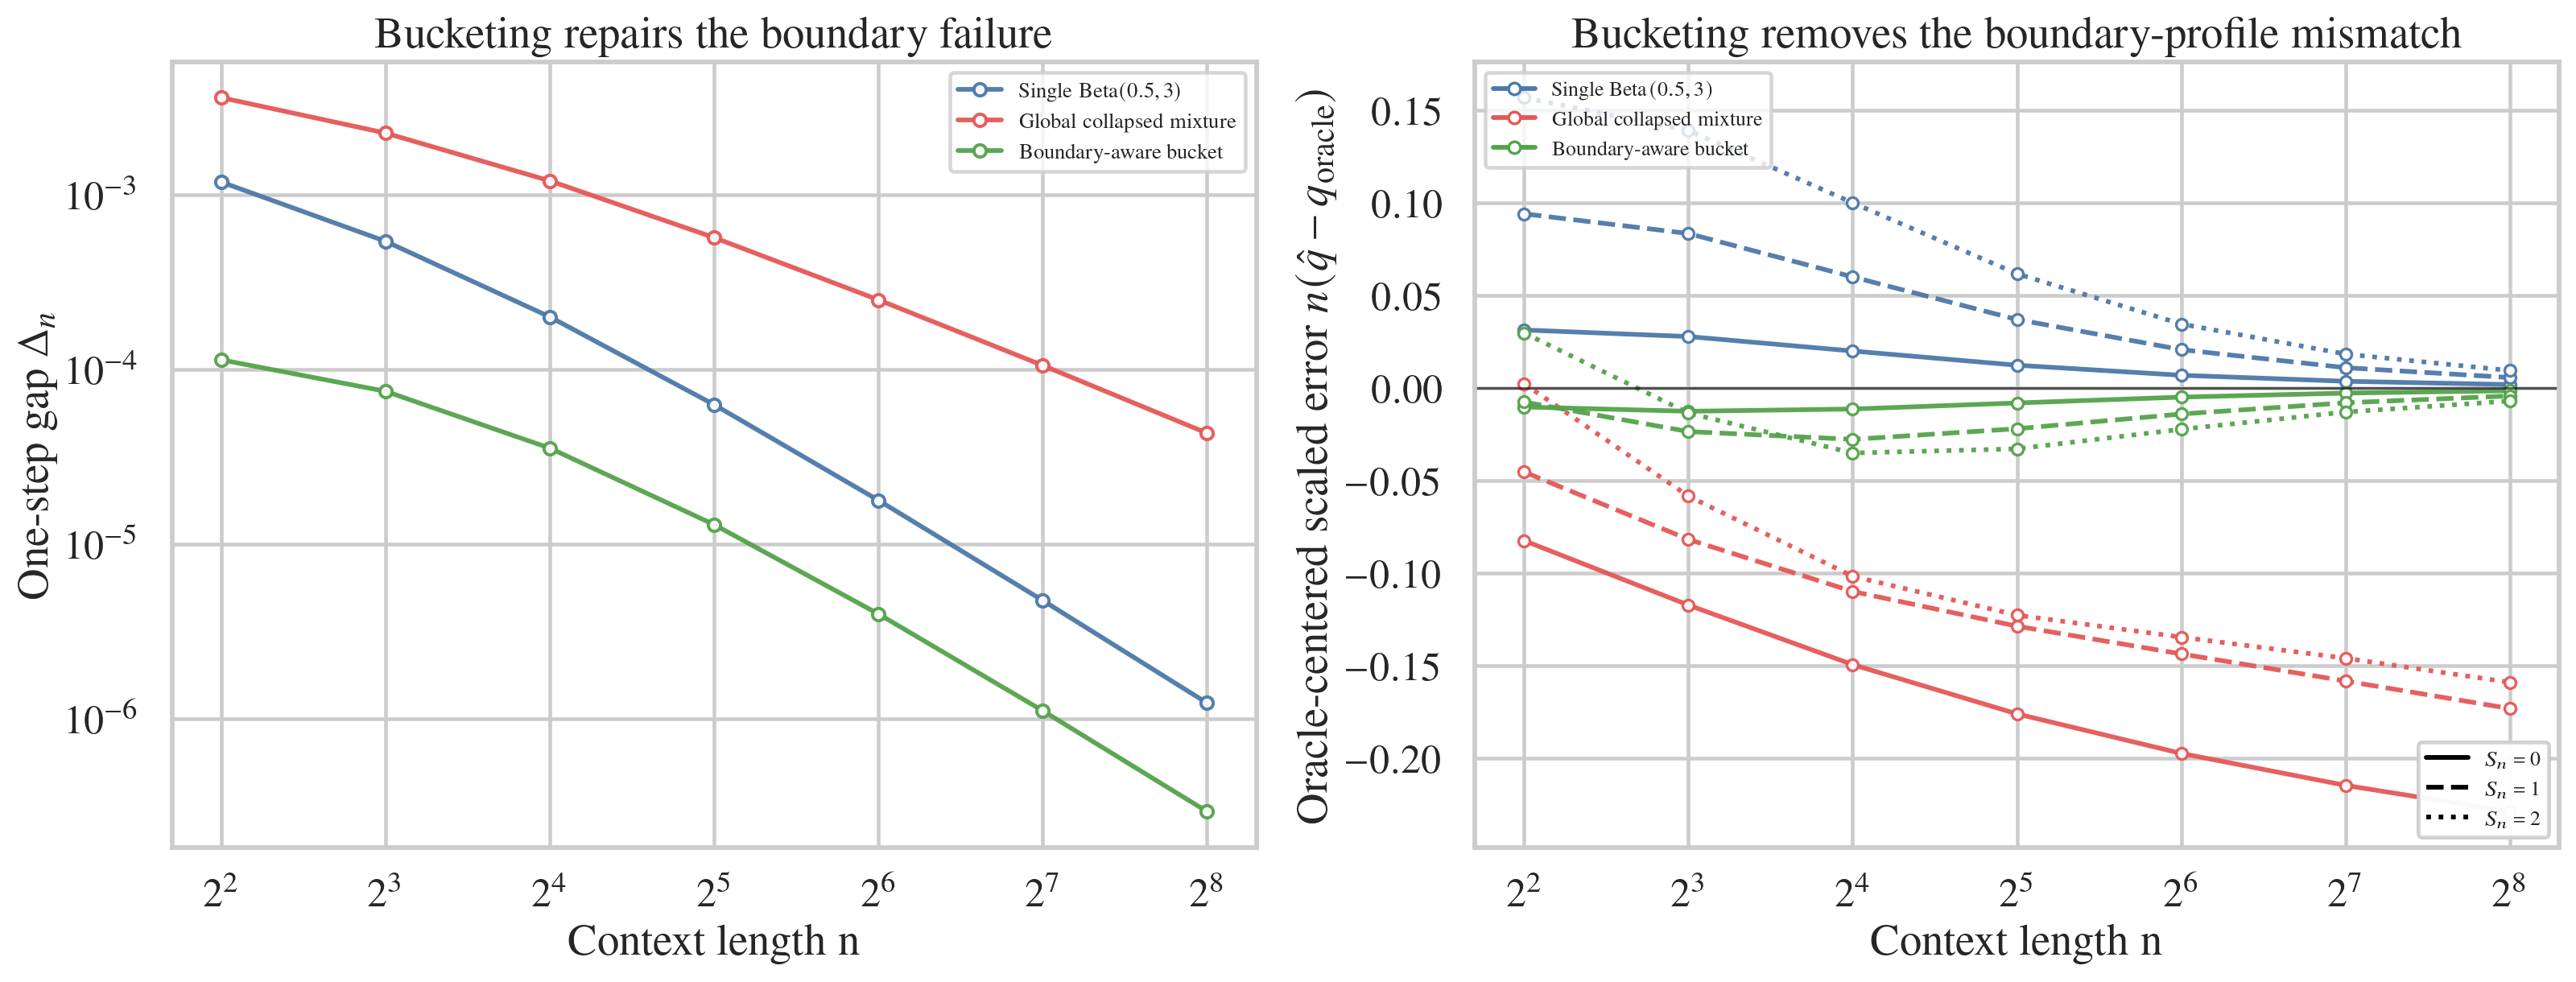
\includegraphics[width=\linewidth]{codes/results/closed_form/figure2_boundary_failure_and_fix.png}
\caption{Closed-form validation of the boundary-profile story on deployment prior $\BetaDist(0.5,4)$. Left: cumulative one-step gap for a strong single constituent prior $\BetaDist(0.5,3)$, a global collapsed mixture, and a profile-matched sublibrary that mixes only the shared-$c=0.5$ component family. Right: oracle-centered small-count profile errors $n(\hat q-q_{\mathrm{oracle}})$ for $S_n\in\{0,1,2\}$. Restricting collapse to the profile-matched sublibrary improves over both the global collapse and the strongest single constituent prior, cutting the exact oracle budget $K_{256}$ from $9.1\times 10^{-2}$ to $2.0\times 10^{-3}$, while the single $\BetaDist(0.5,3)$ prior remains at $2.1\times 10^{-2}$.}
\label{fig:boundary-fix}
\end{figure}

Figure~\ref{fig:boundary-fix} is the main structural ablation for the rare-event story. The global collapsed mixture mixes the right rare-event family with the wrong boundary profile and therefore keeps a substantial small-count mismatch. Restricting the collapse to a profile-matched sublibrary removes most of that mismatch and materially improves the one-step gap. Importantly, the profile-matched predictor is not merely a matched single prior in disguise: it outperforms the strongest single constituent library component because it still hedges \emph{within} the shared profile.

\begin{figure}[t]
\centering
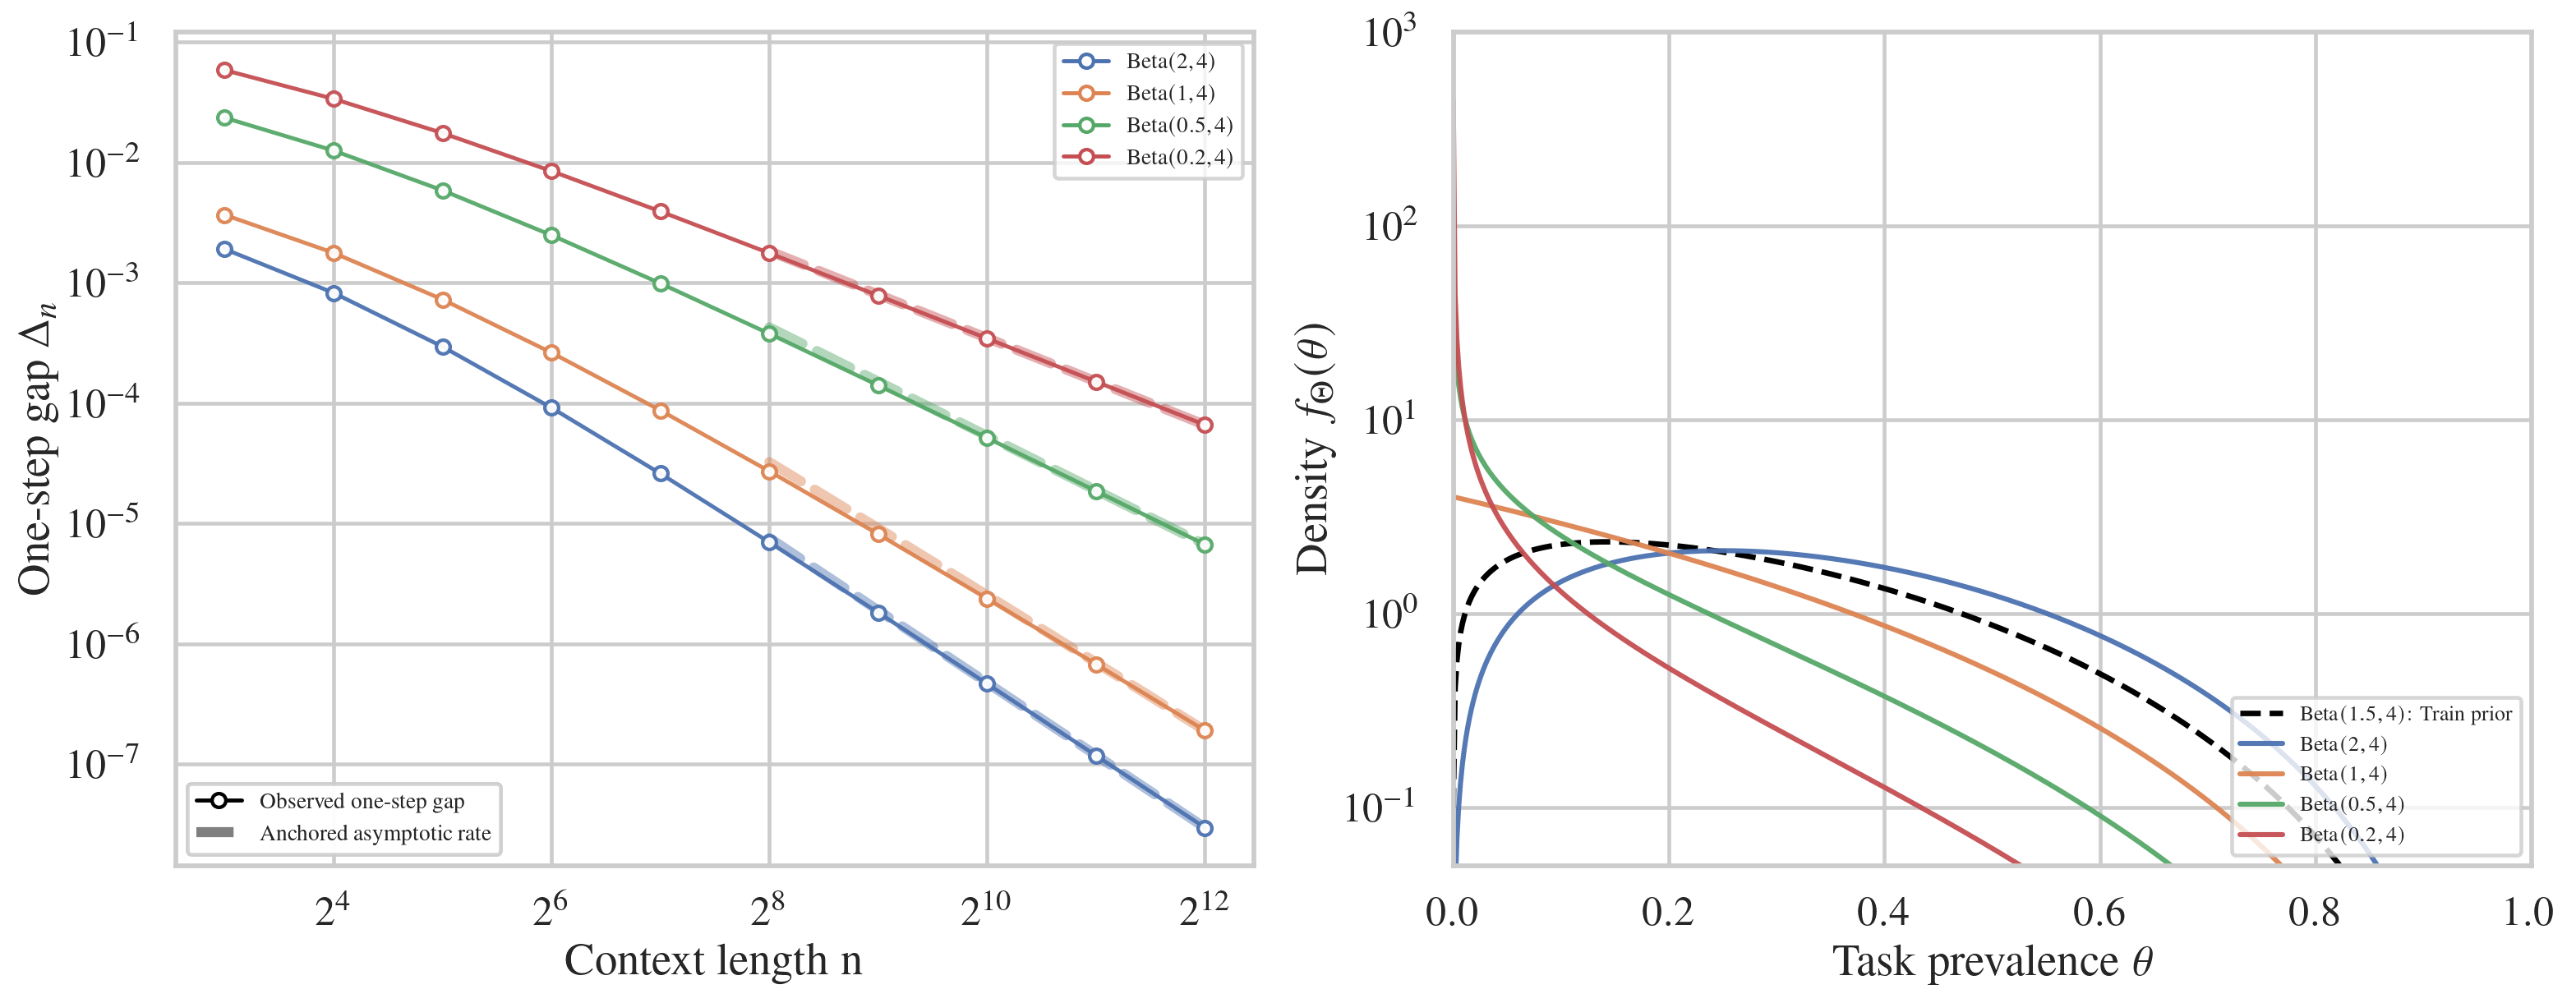
\includegraphics[width=\linewidth]{codes/results/closed_form/figure3_phase_transition.png}
\caption{Closed-form validation of the phase transition in Theorem~\ref{thm:beta}. The left panel shows the observed one-step gap for a fixed training prior $\BetaDist(1.5,4)$ as deployment moves from interior to critical and singular boundary regimes, together with anchored asymptotic reference slopes. The right panel shows the corresponding task-level prevalence priors $f_{\Theta}(\theta)$: as deployment mass shifts toward $\theta\approx 0$, the one-step tail law slows from the regular $n^{-2}$ regime toward the singular $n^{-(1+c)}$ law.}
\label{fig:phase-transition}
\end{figure}

Figure~\ref{fig:phase-transition} validates the rate-level rare-event theory. The fitted tail slopes are approximately $-1.98$ for the interior regime, $-1.81$ for the critical regime, $-1.47$ for $\BetaDist(0.5,4)$, and $-1.19$ for $\BetaDist(0.2,4)$, closely matching the predicted transition from $n^{-2}$ to $(\log n)n^{-2}$ and then to $n^{-(1+c)}$. The right panel shows why: decreasing $c$ shifts more task mass toward near-deterministic rare-event tasks, so small-count boundary events continue to dominate the one-step oracle gap even at large context lengths.

\begin{figure}[t]
\centering
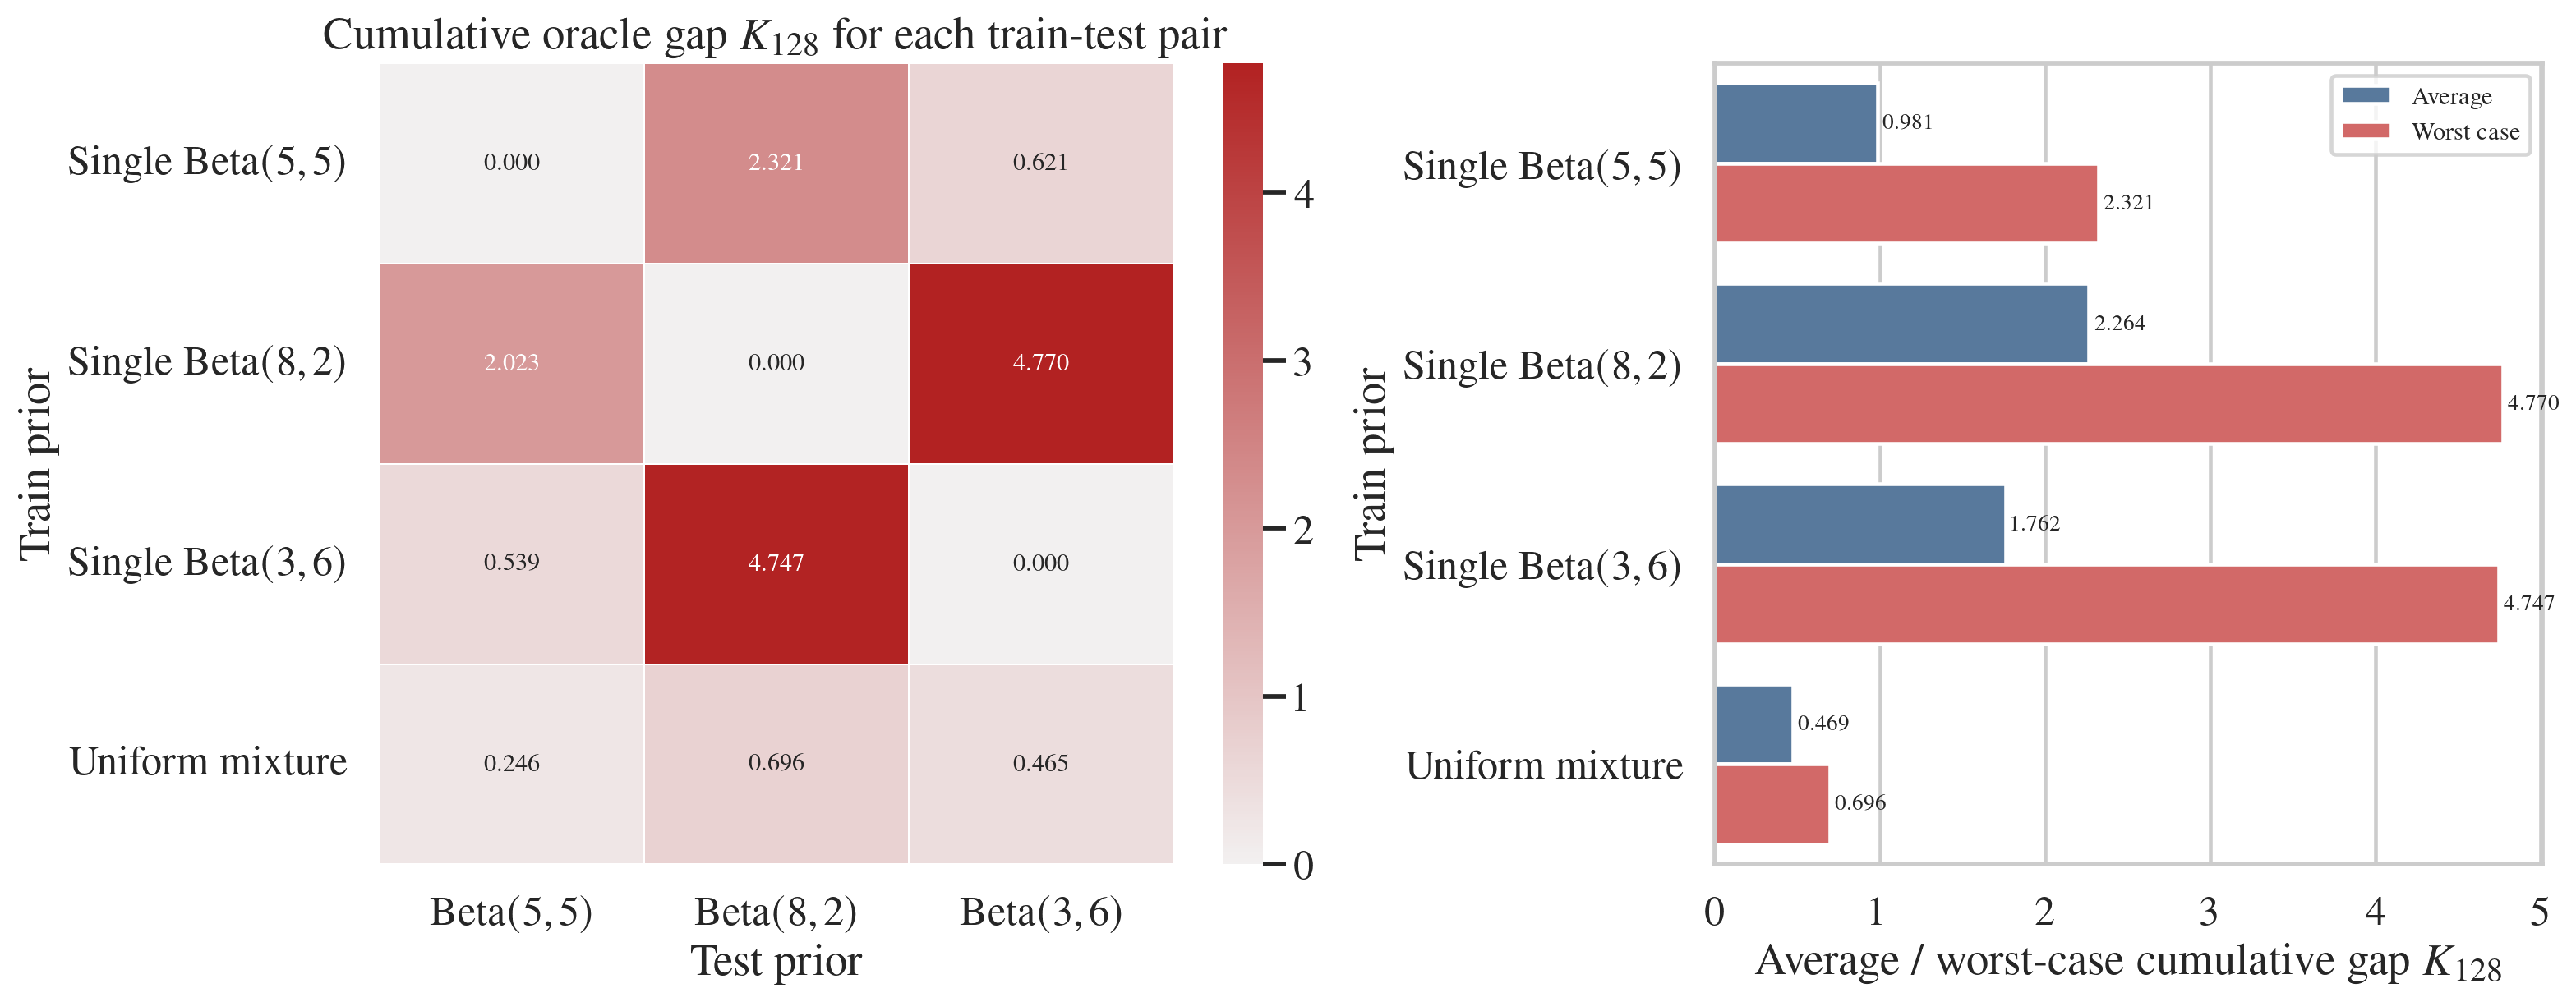
\includegraphics[width=\linewidth]{codes/results/closed_form/figure1_global_hedge.pdf}
\caption{Closed-form validation of Proposition~\ref{thm:mixture}. Three interior train priors are compared against three deployment priors. The left panel reports the cumulative oracle gap $K_{128}$ for each train--test pair; the right panel summarizes average and worst-case regret. The broad mixture sharply improves worst-case robustness, reducing the worst-case gap from $2.32$--$4.77$ for single-family libraries to $0.696$.}
\label{fig:global-hedge}
\end{figure}

Figure~\ref{fig:global-hedge} plays a more limited role: it validates the global hedging claim. On three interior families, a broad mixture is not expected to beat the hindsight-matched specialist on its own family, but it is the best robust default when deployment is unknown. This is the role of Proposition~\ref{thm:mixture}: mixing is the right \emph{coverage} decision even before one decides which family distinctions are unsafe to collapse.

\section{Conclusion}

We can now step back from the theorem chain and answer the motivating question directly: \emph{what makes a PFN prior library unsafe?} The main lesson is asymmetric. Broad mixtures are the right device for coverage, but they are not a license to collapse family structure. The central failure mode is unsafe collapse: a library can be hedge-safe in cumulative KL and still be tail-wrong because its small-count boundary profile is wrong.

\paragraph{1. Cover first, but do not mistake coverage for safety.}
Proposition~\ref{thm:mixture} is the global argument for broad prior libraries: assigning each plausible family positive mass hedges deployment uncertainty. But coverage and merging are different decisions. The relevant object is observable predictive behavior after the prompt, not raw latent generator coordinates.

\paragraph{2. Unsafe collapse is organized by boundary profile.}
Theorem~\ref{thm:beta}, Proposition~\ref{thm:beta-mix}, Proposition~\ref{prop:fixed-count}, Theorem~\ref{thm:boundary-general}, Corollary~\ref{cor:observable-exponent}, Proposition~\ref{prop:stratified-boundary}, Corollary~\ref{cor:stratified-mix}, Corollary~\ref{cor:stratified-shared}, and Section~\ref{sec:imbalance} together say that rare-event mismatch is about small-count boundary profiles, with the exponent as only the first observable summary. In supervised settings the same object becomes query-conditioned and local to the relevant feature stratum. The practical rule is asymmetric: merge within shared-profile classes, but do not collapse across mismatched profiles, preserve the natural prevalence evidence that identifies those profiles, and validate rare-event tails explicitly rather than relying only on average synthetic loss.

\paragraph{3. Label balancing can be an unsafe prompt collapse.}
Proposition~\ref{prop:prompt-transform} says that any prompt transformation incurs exactly the query-conditioned predictive information it deletes, Corollary~\ref{cor:balanced-plus} says that a balanced core is weakly improved by retaining the deleted evidence as a side channel, Proposition~\ref{prop:balanced-useless} shows that a perfectly balanced prompt can be asymptotically no better than no prompt at all for prevalence learning, and Theorem~\ref{thm:balancing-counterexample} shows that label-balanced prompts can induce score distortions that are not mere intercept shifts. So for PFNs the relevant question is not ``should the loss be class-balanced?'' but ``which prompt statistics are safe to delete?'' In extreme imbalance settings, a $1{:}1$ prompt without an accompanying base-rate or query-local statistic can erase the very evidence needed to identify the correct latent family.

\paragraph{4. Merge only when prompt-conditioned predictive distinctiveness is small.}
Proposition~\ref{prop:prompt-opt} and Corollary~\ref{cor:js} say that the right split/merge object is the prompt-conditioned generalized Jensen--Shannon divergence, not unconditional diversity. Families should be merged only when that prompt-conditioned geometry is small; otherwise the irreducible collapse cost remains visible after the prompt.

\paragraph{Limitations.}

This paper is theory-first. The sharpest results are oracle statements about what no architecture can undo unless the synthetic prior itself changes. The oracle identities in Section~\ref{sec:oracle-design} identify the target quantity $\I(F;Y\mid O)$, but they do not by themselves provide an automatic estimator of it or a complete procedure for selecting among candidate family collapses. Our empirical section reports only exact closed-form validations, and those validations currently target the analytically solvable $K=1$ special case. Finally, the sharpest closed-form rare-event rates remain in one-dimensional Bernoulli prevalence models, while the supervised extension in Section~\ref{sec:stratified} is developed only for finite strata rather than fully continuous covariates, and the regular benchmark relies on a one-posterior quadratic-tilt regime made explicit in Appendix~\ref{app:regular-proofs}.

\paragraph{Discussion.}

The message is deliberately simple. Unsafe collapse, not insufficient library breadth, is the core PFN prior failure mode. Mix broadly to hedge globally. Do not collapse across boundary profiles just because average synthetic loss looks benign. In supervised settings, preserve the query-conditioned boundary evidence carried by local counts near the query. Merge only when the prompt-conditioned predictive geometry certifies that doing so is safe. And do not balance away the prevalence evidence that identifies the dangerous rare-event regimes in the first place.

\section*{Acknowledgments}

This submission is anonymized for review.

\appendix

\section{Proofs}

\subsection{Proof of Proposition~\ref{prop:prompt-transform}}

\begin{proof}
By definition of Bayes risk,
\[
R(q_{\widetilde O})-R(q_O)
=
H(Y_{n+1}\mid \widetilde H_n,X_{n+1})-H(Y_{n+1}\mid H_n,X_{n+1})
=
\I(Y_{n+1};H_n\mid \widetilde H_n,X_{n+1}).
\]
Because $O_n=(X_{n+1},H_n)$ and $\widetilde O_n=(X_{n+1},\widetilde H_n)$, the same quantity can be rewritten as
\[
\I(Y_{n+1};H_n\mid \widetilde H_n,X_{n+1})
=
H(Y_{n+1}\mid \widetilde O_n)-H(Y_{n+1}\mid O_n)
=
\I(Y_{n+1};O_n\mid \widetilde O_n),
\]
because $Y_{n+1}\to O_n\to \widetilde O_n$ is a Markov chain. If $H_n=(\widetilde H_n,C_n)$ almost surely, then the chain rule gives
\[
\I(Y_{n+1};H_n\mid \widetilde H_n,X_{n+1})
=
\I(Y_{n+1};\widetilde H_n,C_n\mid \widetilde H_n,X_{n+1})
=
\I(Y_{n+1};C_n\mid \widetilde H_n,X_{n+1}),
\]
as claimed.
\end{proof}

\subsection{Proof of Corollary~\ref{cor:balanced-plus}}

\begin{proof}
Apply Proposition~\ref{prop:prompt-transform} with the transformed prompt $\widetilde O_n$ taken to be $\widetilde O_n^{\mathrm{bal}}=(X_{n+1},\widetilde H_n^{\mathrm{bal}})$ and the refined prompt taken to be
\[
\bar O_n=(X_{n+1},\widetilde H_n^{\mathrm{bal}},C_n).
\]
Since $\bar O_n$ is a refinement of $\widetilde O_n^{\mathrm{bal}}$, the proposition gives
\[
R(q_{\widetilde O^{\mathrm{bal}}})-R(q_{\bar O})
=
\I(Y_{n+1};C_n\mid \widetilde H_n^{\mathrm{bal}},X_{n+1}).
\]
Nonnegativity of conditional mutual information yields the weak domination claim. In the finite-strata model, taking $C_n=(N_{n,k},S_{n,k})$ for the realized query stratum $k$ gives the stated canonical choice.
\end{proof}

\subsection{Proof of Proposition~\ref{prop:balanced-useless}}

\begin{proof}
By construction $\widetilde O_m$ is a random permutation of exactly $m$ zeros and $m$ ones, so its law is the same for every $\theta$. Hence $\widetilde O_m \perp\!\!\!\perp \theta$, and
\[
q_m^{\mathrm{bal}}(1\mid \widetilde O_m)
=
\Pbb(Y_*=1\mid \widetilde O_m)
=
\Pbb(Y_*=1)
=
\E[\theta]
=
\frac{c}{c+d}.
\]
Under the natural prompt, conjugacy gives
\[
q_{2m}^{\mathrm{nat}}(1\mid O_{2m})
=
\E[\theta\mid O_{2m}]
=
\frac{c+S_{2m}}{c+d+2m}.
\]
Since $S_{2m}/(2m)\to \theta$ almost surely, it follows that $q_{2m}^{\mathrm{nat}}(1\mid O_{2m})\to \theta$ almost surely.

For the balanced prompt risk, let $\bar \theta:=c/(c+d)$. Because $Y_*\mid \theta \sim \Ber(\theta)$,
\[
R_m^{\mathrm{bal}}
=
\E\bigl[-\theta\log \bar\theta -(1-\theta)\log(1-\bar\theta)\bigr]
=
h(\bar\theta).
\]
For the natural prompt, Bayes optimality gives
\[
R_{2m}^{\mathrm{nat}}
=
H(Y_{2m+1}\mid O_{2m})
=
\E\!\left[h\!\left(q_{2m}^{\mathrm{nat}}(1\mid O_{2m})\right)\right].
\]
Because $0\le h\le \log 2$ and $q_{2m}^{\mathrm{nat}}(1\mid O_{2m})\to \theta$ almost surely, bounded convergence yields
\[
R_{2m}^{\mathrm{nat}}\to \E[h(\theta)].
\]
Finally, for $Y\mid \theta\sim \Ber(\theta)$ and marginal $Y\sim \Ber(\bar \theta)$,
\[
\I(\theta;Y)
=
H(Y)-H(Y\mid \theta)
=
h(\bar\theta)-\E[h(\theta)].
\]
This proves the limit identity.
\end{proof}

\subsection{Proof of Theorem~\ref{thm:balancing-counterexample}}

\begin{proof}
Because $C=\ind\{F=A\}$ is part of the full prompt, the full-prompt Bayes predictor identifies the realized family exactly. Under the realized family $F=A$,
\[
q_O(1\mid x_1,F=A)=0.05,
\qquad
q_O(1\mid x_2,F=A)=0.001,
\]
so the full-prompt Bayes ordering is $x_1 \succ x_2$.

By construction, the balanced prompt $\widetilde O=(U,X_*)$ omits $C$ and $U$ is conditionally independent of $F$, so the posterior on $F$ remains uniform:
\[
\Pbb(F=A\mid \widetilde O)=\Pbb(F=B\mid \widetilde O)=\frac{1}{2}.
\]
Hence the balanced-prompt Bayes predictor is the family average
\[
q_{\widetilde O}(1\mid x)
=
\frac{1}{2}\Pbb(Y_*=1\mid x,F=A)
+
\frac{1}{2}\Pbb(Y_*=1\mid x,F=B).
\]
Therefore
\[
q_{\widetilde O}(1\mid x_1)
=
\frac{0.05+10^{-4}}{2}
=
0.02505,
\]
\[
q_{\widetilde O}(1\mid x_2)
=
\frac{0.001+0.9}{2}
=
0.4505.
\]
So the balanced-prompt ordering is $x_2 \succ x_1$, the reverse of the full-prompt Bayes ordering under family $A$.

Any global threshold, temperature scaling, or intercept shift is a monotone transformation of the score, so it cannot undo a strict ranking reversal. This proves the non-thresholdability claim.

For the excess log risk under family $A$, condition on $X_*$ and average:
\[
R_A(q_{\widetilde O})-R_A(q_O)
=
\frac{1}{2}\klb(0.05,0.02505)
+
\frac{1}{2}\klb(0.001,0.4505),
\]
which evaluates numerically to approximately $3.00\times 10^{-1}$.
\end{proof}

\subsection{Proof of Theorem~\ref{thm:exact}}

\begin{proof}
By definition,
\begin{align*}
K_{n+1}-K_n
&=
\E_{m_{\te}^{n+1}}
\left[
\log\frac{m_{\te}^{n+1}(Z_{1:n+1})}{m_{\tr}^{n+1}(Z_{1:n+1})}
-
\log\frac{m_{\te}^{n}(Z_{1:n})}{m_{\tr}^{n}(Z_{1:n})}
\right] \\
&=
\E_{m_{\te}^{n+1}}
\left[
\log
\frac{
m_{\te}^{n+1}(Z_{1:n+1}) / m_{\te}^{n}(Z_{1:n})
}{
m_{\tr}^{n+1}(Z_{1:n+1}) / m_{\tr}^{n}(Z_{1:n})
}
\right] \\
&=
\E_{m_{\te}^{n+1}}
\left[
\log
\frac{
q_n^{\te}(Z_{n+1}\mid Z_{1:n})
}{
q_n^{\tr}(Z_{n+1}\mid Z_{1:n})
}
\right]
=
\Delta_n.
\end{align*}
Conditioning on $Z_{1:n}$ under $m_{\te}^{n+1}$ yields
\[
\Delta_n
=
\E_{m_{\te}^{n}}
\Bigl[
\KL\bigl(
q_n^{\te}(\cdot\mid Z_{1:n})
\;\|\;
q_n^{\tr}(\cdot\mid Z_{1:n})
\bigr)
\Bigr].
\]

Define joint laws on $(t,Z_{1:n})$:
\[
J_{\te}(\dd t,\dd z_{1:n})
:=
\pi_{\te}(\dd t)\prod_{i=1}^n P_t(\dd z_i),
\qquad
J_{\tr}(\dd t,\dd z_{1:n})
:=
\pi_{\tr}(\dd t)\prod_{i=1}^n P_t(\dd z_i).
\]
Because the conditional law of $Z_{1:n}$ given $t$ is the same under both,
\[
\KL(J_{\te}\,\|\,J_{\tr})=\KL(\pi_{\te}\,\|\,\pi_{\tr}).
\]
Applying the chain rule for KL with the marginal on $Z_{1:n}$ gives
\begin{align*}
\KL(J_{\te}\,\|\,J_{\tr})
&=
\KL(m_{\te}^{n}\,\|\,m_{\tr}^{n}) \\
&\qquad
+ \E_{m_{\te}^{n}}
\Bigl[
\KL\bigl(
\pi_{\te}(\cdot\mid Z_{1:n})
\;\|\;
\pi_{\tr}(\cdot\mid Z_{1:n})
\bigr)
\Bigr] \\
&=
K_n + D_n.
\end{align*}
Hence
\[
K_n=\KL(\pi_{\te}\,\|\,\pi_{\tr})-D_n.
\]
Subtracting the same identity at $n+1$ and using Theorem~\ref{thm:exact},
\[
\Delta_n = K_{n+1}-K_n = D_n-D_{n+1}.
\]
Finally,
\[
\sum_{n=0}^{N-1}\Delta_n
=
K_N-K_0.
\]
Since $K_0=0$ and $K_N\le \KL(\pi_{\te}\,\|\,\pi_{\tr})$, the cumulative bound follows.
\end{proof}

\subsection{Proof of Proposition~\ref{thm:mixture}}
\label{app:exact-proofs}

\begin{proof}
The equality
\[
\sum_{n=0}^{N-1}\Delta_n(\pi_\alpha,\pi_\lambda)
=
\KL(m_\alpha^N\,\|\,m_\lambda^N)
\]
is immediate from Theorem~\ref{thm:exact} by telescoping from $n=0$ to $N-1$.

For the upper bound, introduce the latent family index $J\in\{1,\dots,M\}$ and define
\[
\widetilde P_\alpha(j,z_{1:N}) := \alpha_j m_{\pi_j}^N(z_{1:N}),
\qquad
\widetilde P_\lambda(j,z_{1:N}) := \lambda_j m_{\pi_j}^N(z_{1:N}).
\]
Because the conditional law of $Z_{1:N}$ given $J=j$ is the same under both,
\[
\KL(\widetilde P_\alpha\,\|\,\widetilde P_\lambda)
=
\KL(\alpha\,\|\,\lambda).
\]
Marginalizing out $J$ maps $(J,Z_{1:N})$ to $Z_{1:N}$, and the corresponding marginals are exactly $m_\alpha^N$ and $m_\lambda^N$. By data processing,
\[
\KL(m_\alpha^N\,\|\,m_\lambda^N)
\le
\KL(\widetilde P_\alpha\,\|\,\widetilde P_\lambda)
=
\KL(\alpha\,\|\,\lambda).
\]
The single-family specialization is obtained by setting $\alpha=e_j$.
\end{proof}

\subsection{Proof of Proposition~\ref{prop:prompt-opt}}

\begin{proof}
Let $q_{\mathrm{aware}}(y\mid O_n,F)=P(Y_{n+1}=y\mid O_n,F)$ and
$q_{\mathrm{coll}}(y\mid O_n)=P(Y_{n+1}=y\mid O_n)$. For any predictive law $r(\cdot\mid O_n)$ measurable with respect to $O_n$, add and subtract the collapsed risk:
\begin{align*}
&\E[-\log r(Y_{n+1}\mid O_n)]
-\E[-\log q_{\mathrm{aware}}(Y_{n+1}\mid O_n,F)] \\
&=
\Bigl(
\E[-\log r(Y_{n+1}\mid O_n)]
-\E[-\log q_{\mathrm{coll}}(Y_{n+1}\mid O_n)]
\Bigr) \\
&\qquad +
\Bigl(
\E[-\log q_{\mathrm{coll}}(Y_{n+1}\mid O_n)]
-\E[-\log q_{\mathrm{aware}}(Y_{n+1}\mid O_n,F)]
\Bigr).
\end{align*}
Conditioning on $O_n$ turns the first bracket into
\[
\E\!\left[
-\log r(Y_{n+1}\mid O_n)
+\log q_{\mathrm{coll}}(Y_{n+1}\mid O_n)
\;\middle|\;
O_n
\right]
=
\KL\bigl(
q_{\mathrm{coll}}(\cdot\mid O_n)
\;\|\;
r(\cdot\mid O_n)
\bigr).
\]
The second bracket equals
\[
H(Y_{n+1}\mid O_n)-H(Y_{n+1}\mid O_n,F)
=
\I(F;Y_{n+1}\mid O_n).
\]
Averaging proves the decomposition, and setting $r=q_{\mathrm{coll}}$ gives the final display.
\end{proof}

\subsection{Proof of Corollary~\ref{cor:js}}

\begin{proof}
Condition on $O_n=o$. The conditional law of $F$ then has weights $w(o)$ and mixture predictive $q_{\mathrm{coll}}(\cdot\mid o)$. Therefore
\[
\I(F;Y_{n+1}\mid O_n=o)
=
\sum_{j=1}^M w_j(o)\,
\KL\bigl(
q_j(\cdot\mid o)
\;\|\;
q_{\mathrm{coll}}(\cdot\mid o)
\bigr)
=
\JS_{w(o)}(q_1,\dots,q_M).
\]
Average over $O_n$ and invoke Proposition~\ref{prop:prompt-opt}.
\end{proof}

\subsection{Proof of Proposition~\ref{prop:regular}}
\label{app:regular-proofs}

\begin{assumption}[One-posterior regularity]
\label{ass:bvm}
Tasks are parameterized by $\theta\in\Theta\subset\Rbb^p$, where $\Theta$ is open and $Z_i\mid \theta \sim P_\theta$ i.i.d. Let $\pi_{\tr}$ and $\pi_{\te}$ have positive densities on $\Theta$ and define
\[
g(\theta):=\log \frac{\pi_{\te}(\theta)}{\pi_{\tr}(\theta)},
\qquad
u(\theta):=\nabla g(\theta),
\qquad
I(\theta):=\text{Fisher information of }P_\theta.
\]
Assume $g\in C^3(\Theta)$. If $\theta_0$ generates $Z_{1:n}$ and
\[
\Pi_{\tr,n}:=\pi_{\tr}(\cdot\mid Z_{1:n}),
\]
then:
\begin{enumerate}[leftmargin=18pt]
\item there exist measurable envelopes $L,M:\Theta\to[1,\infty)$ such that, for $\pi_{\te}$-almost every $\theta_0$,
\[
\sup_{\|\vartheta-\theta_0\|\le 1}
\max\!\left\{
\|\nabla^2 g(\vartheta)\|,
\|\nabla^3 g(\vartheta)\|
\right\}
\le
L(\theta_0),
\]
\[
\sup_{n\ge 1}
\E_{Z_{1:n}\mid \theta_0}
\E_{\Pi_{\tr,n}}
\|\sqrt n(\Theta-\theta_0)\|^3
\le
M(\theta_0),
\]
and
\[
\E_{\theta\sim\pi_{\te}}
\bigl[(1+\|u(\theta)\|^3)L(\theta)M(\theta)\bigr]
<\infty;
\]
\item the posterior covariance satisfies the weighted $L^1$ convergence
\[
\E_{\theta_0\sim\pi_{\te}}
\E_{Z_{1:n}\mid \theta_0}
\left|
u(\theta_0)^\top
\Bigl(
n\,\Var_{\Pi_{\tr,n}}(\Theta)-I(\theta_0)^{-1}
\Bigr)
u(\theta_0)
\right|
\to 0.
\]
\end{enumerate}
These conditions are the one-posterior BvM input we need: local quadratic control of the posterior tilt $g$, posterior third-moment localization at scale $n^{-1/2}$, and integrable weighted covariance convergence for the training posterior.
\end{assumption}

\begin{proof}
Fix the true parameter $\theta_0$ and write $\Pi_n:=\Pi_{\tr,n}=\pi_{\tr}(\cdot\mid Z_{1:n})$.
Because the likelihood is the same under both priors, Bayes' rule gives the exact posterior tilt identity
\[
\frac{\dd \pi_{\te}(\cdot\mid Z_{1:n})}{\dd \Pi_n}(\theta)
=
\frac{e^{g(\theta)}}{\E_{\Pi_n}e^{g(\Theta)}}.
\]
Hence the posterior KL at the realized dataset equals
\begin{align*}
D_n(Z_{1:n})
&:=
\KL\bigl(
\pi_{\te}(\cdot\mid Z_{1:n})
\;\|\;
\pi_{\tr}(\cdot\mid Z_{1:n})
\bigr) \\
&=
\E_{\pi_{\te}(\cdot\mid Z_{1:n})} g(\Theta)
- \log \E_{\Pi_n} e^{g(\Theta)}.
\end{align*}

Subtract the constant $g(\theta_0)$ and define
\[
X_n:=g(\Theta)-g(\theta_0),
\qquad
\psi_n(\lambda):=\log \E_{\Pi_n} e^{\lambda X_n}.
\]
Then
\[
D_n(Z_{1:n}) = \psi_n'(1)-\psi_n(1).
\]

A third-order Taylor expansion of $g$ around $\theta_0$ gives
\[
X_n
=
u(\theta_0)^\top(\Theta-\theta_0)
 + R_n,
\qquad
|R_n|
\le
C L(\theta_0)\|\Theta-\theta_0\|^2
\]
for a universal constant $C$. By Assumption~\ref{ass:bvm}(1) and H\"older's inequality,
\[
\E_{Z_{1:n}\mid \theta_0}\E_{\Pi_n}|R_n|
\le
C L(\theta_0) M(\theta_0)^{2/3} n^{-1},
\]
and similarly
\[
\E_{Z_{1:n}\mid \theta_0}\E_{\Pi_n}|X_n|^3
\le
C (1+\|u(\theta_0)\|^3)L(\theta_0)M(\theta_0)\,n^{-3/2}.
\]
Thus $X_n=o_{L^3(\Pi_n)}(1)$ on average under the data law. Conditioning on a realized dataset and using the standard scalar cumulant expansion with third-moment remainder, there is a deterministic remainder $\rho_n(\lambda)$ such that, uniformly for $\lambda\in[0,1]$,
\[
\psi_n(\lambda)
=
\lambda m_n + \frac{\lambda^2}{2}v_n + O_{P_{\theta_0}}(n^{-3/2}),
\]
where
\[
m_n:=\E_{\Pi_n}X_n,
\qquad
v_n:=\Var_{\Pi_n}(X_n).
\]
More explicitly, the remainder satisfies
\[
\E_{Z_{1:n}\mid \theta_0}\sup_{\lambda\in[0,1]}|\rho_n(\lambda)|
\le
C (1+\|u(\theta_0)\|^3)L(\theta_0)M(\theta_0)\,n^{-3/2},
\]
so the displayed $O(n^{-3/2})$ term is $L^1$-controlled rather than merely formal.
Consequently,
\[
\psi_n'(1)-\psi_n(1)
=
\frac{1}{2}v_n + O_{L^1(P_{\theta_0})}(n^{-3/2}).
\]

Applying the same Taylor expansion inside the variance gives
\[
v_n
=
u(\theta_0)^\top \Var_{\Pi_n}(\Theta)\,u(\theta_0)
+ O_{L^1(P_{\theta_0})}(n^{-3/2}).
\]
Combining the last two displays gives
\[
D_n(Z_{1:n})
=
\frac{1}{2}\,
u(\theta_0)^\top \Var_{\Pi_n}(\Theta)\,u(\theta_0)
+ O_{L^1(P_{\theta_0})}(n^{-3/2}).
\]

Now average over $\theta_0\sim\pi_{\te}$ and the data. The integrability condition in Assumption~\ref{ass:bvm}(1) makes the $n^{-3/2}$ remainder uniformly integrable after averaging over $\theta_0$, so its contribution is $o(n^{-1})$. Assumption~\ref{ass:bvm}(2) then yields
\[
D_n
=
\frac{1}{2n}\,
\E_{\theta\sim\pi_{\te}}
\bigl[
u(\theta)^\top I(\theta)^{-1}u(\theta)
\bigr]
+ o(n^{-1}).
\]
Theorem~\ref{thm:exact} then gives
\[
\Delta_n
=
D_n-D_{n+1}
=
\frac{1}{2n(n+1)}\,
\E_{\theta\sim\pi_{\te}}
\bigl[
u(\theta)^\top I(\theta)^{-1}u(\theta)
\bigr]
+ o(n^{-2}).
\qedhere
\]
\end{proof}

\subsection{Proof of Theorem~\ref{thm:beta}}
\label{app:beta-proofs}

We use the shorthand
\[
p_n(s) := \frac{c+s}{c+d+n},
\qquad
q_n(s) := \frac{a+s}{a+b+n},
\qquad
r_n(\theta) := \E_{S\sim \Bin(n,\theta)}[\klb(p_n(S),q_n(S))].
\]

\begin{lemma}[Integral representation]
\label{lem:beta-integral}
For every $n\ge 0$,
\[
\Delta_n
=
\frac{1}{B(c,d)}
\int_0^1
\theta^{c-1}(1-\theta)^{d-1}
r_n(\theta)\,\dd\theta.
\]
\end{lemma}

\begin{proof}
Under the deployment prior $\theta\sim \BetaDist(c,d)$, the sufficient statistic $S_n$ has Beta--Binomial distribution:
\[
\Pbb(S_n=s)
=
\binom{n}{s}
\frac{B(c+s,d+n-s)}{B(c,d)}.
\]
Therefore
\[
\Delta_n
=
\sum_{s=0}^n \Pbb(S_n=s)\,\klb(p_n(s),q_n(s)).
\]
Expanding the Beta--Binomial law as a Beta mixture of Binomials yields the integral representation.
\end{proof}

\begin{lemma}[Pointwise upper bound near the left boundary]
\label{lem:left-upper}
Assume $a,b,c,d>0$. There exists a constant $C>0$ such that for all $n\ge 1$ and $\theta\in[0,1]$,
\[
r_n(\theta) \le \frac{C}{n(1+n\theta)}.
\]
\end{lemma}

\begin{proof}
For Bernoulli KL,
\[
\klb(u,v) \le \frac{(u-v)^2}{v(1-v)}
\qquad
u,v\in(0,1).
\]
Now
\[
p_n(s)-q_n(s)
=
\frac{(c-a)n + (a+b-c-d)s + cb-ad}
{(n+c+d)(n+a+b)},
\]
so $|p_n(s)-q_n(s)|\le C_1/n$ uniformly in $s\in\{0,\dots,n\}$. Also
\[
q_n(s)=\frac{a+s}{a+b+n}\ge \frac{a+s}{n+a+b},
\qquad
1-q_n(s)\ge \frac{b+n-s}{n+a+b}\ge \frac{b}{n+a+b}.
\]
Hence
\[
\klb(p_n(s),q_n(s))
\le
\frac{C_2}{n(a+s)}.
\]
Taking the expectation with respect to $S\sim \Bin(n,\theta)$ gives
\[
r_n(\theta)\le \frac{C_2}{n}\E\frac{1}{a+S}.
\]
Because $(a+s)^{-1}\le C_3(1+s)^{-1}$ for $a>0$, it suffices to bound $\E[(1+S)^{-1}]$. A standard binomial identity gives
\[
\E\frac{1}{1+S}
=
\frac{1-(1-\theta)^{n+1}}{(n+1)\theta}
\le
\frac{C_4}{1+n\theta},
\]
with the convention that the left-hand side equals $1$ at $\theta=0$. Combining the estimates proves the lemma.
\end{proof}

\begin{lemma}[Pointwise lower bound near the left boundary]
\label{lem:left-lower}
Assume $a\neq c$ and $d>0$. Then there exist constants $\theta_0\in(0,1/4)$, $n_0\ge 1$, and $c_0>0$ such that for all $n\ge n_0$ and all $\theta\in[8/n,\theta_0]$,
\[
r_n(\theta) \ge \frac{c_0}{n^2\theta}.
\]
\end{lemma}

\begin{proof}
Let
\[
A:=c-a,
\qquad
B:=a+b-c-d,
\qquad
C:=cb-ad.
\]
Choose $\theta_0>0$ such that $|B|\theta_0 \le |A|/8$ and $(2+\theta_0)\theta_0\le 1/2$. For $\theta\in[8/n,\theta_0]$, define
\[
E_\theta := \left\{\,|S-n\theta|\le \frac{n\theta}{2}\,\right\},
\qquad S\sim \Bin(n,\theta).
\]
Since $\Var(S)=n\theta(1-\theta)\le n\theta$, Chebyshev's inequality yields
\[
\Pbb(E_\theta^c)
\le
\frac{4\Var(S)}{n^2\theta^2}
\le
\frac{4}{n\theta}
\le
\frac{1}{2},
\]
so $\Pbb(E_\theta)\ge 1/2$.

On $E_\theta$, we have $s\in[n\theta/2,3n\theta/2]$, hence
\[
|A|n-|B|s-|C|
\ge
|A|n - \frac{3}{2}|B|n\theta - |C|
\ge
\frac{|A|}{2}n
\]
for all $n\ge n_0$ sufficiently large. Therefore
\[
|p_n(s)-q_n(s)|
\ge
\frac{|A|}{4n}
\qquad\text{on }E_\theta.
\]
Also, on $E_\theta$ and for $n\ge n_0$,
\[
p_n(s)\le \frac{c+3n\theta/2}{n+c+d}\le 2\theta,
\qquad
q_n(s)\le \frac{a+3n\theta/2}{n+a+b}\le 2\theta.
\]
Because $\theta\le\theta_0<1/4$, both probabilities are at most $1/2$. For fixed $v\in(0,1)$, the function $u\mapsto \klb(u,v)$ has second derivative
\[
\frac{1}{u(1-u)}.
\]
On the interval $u\in[0,2\theta]$ with $\theta\le 1/4$, this derivative is at least $(2\theta)^{-1}$. Since $\klb(v,v)=0$ and the first derivative at $u=v$ is zero, Taylor's theorem gives
\[
\klb(u,v)\ge \frac{(u-v)^2}{4\theta}
\qquad\text{whenever }u,v\in[0,2\theta].
\]
Applying this with $u=p_n(s)$ and $v=q_n(s)$ on $E_\theta$,
\[
\klb(p_n(s),q_n(s))
\ge
\frac{A^2}{64\,n^2\theta}.
\]
Taking expectations and using $\Pbb(E_\theta)\ge 1/2$ proves the lemma.
\end{proof}

\begin{proof}
The exact predictive formula and the Beta--Binomial representation are immediate from conjugacy and Lemma~\ref{lem:beta-integral}.

For part (1), the Bernoulli model has Fisher information
\[
I(\theta)=\frac{1}{\theta(1-\theta)}.
\]
When $c,d>1$, the deployment prior is interior enough for the regular benchmark from Section~\ref{sec:regular} to apply, with
\[
u(\theta)
=
\frac{c-a}{\theta}
- \frac{d-b}{1-\theta}.
\]
Therefore
\[
u(\theta)^2 I(\theta)^{-1}
=
\frac{(c-a)^2(1-\theta)}{\theta}
+
\frac{(d-b)^2\theta}{1-\theta}
-2(c-a)(d-b).
\]
Under $\theta\sim\BetaDist(c,d)$,
\[
\E\frac{1-\theta}{\theta}=\frac{d}{c-1},
\qquad
\E\frac{\theta}{1-\theta}=\frac{c}{d-1},
\]
which yields the constant $C_{a,b,c,d}$ and the expansion
\[
\Delta_n = \frac{C_{a,b,c,d}}{2n^2}+o(n^{-2}).
\]

For part (2), assume $0<c<1<d$ and $a\neq c$. By Lemma~\ref{lem:left-upper},
\[
\Delta_n
\le
\frac{C}{B(c,d)}
\int_0^1
\frac{\theta^{c-1}(1-\theta)^{d-1}}{n(1+n\theta)}
\dd\theta.
\]
Split the integral at $\theta=1/n$. Using $(1-\theta)^{d-1}\le 1$,
\begin{align*}
\Delta_n
&\le
\frac{C}{n}\int_0^{1/n}\theta^{c-1}\dd\theta
+
\frac{C}{n^2}\int_{1/n}^{1}\theta^{c-2}\dd\theta \\
&\le
C' n^{-(1+c)}.
\end{align*}
For the lower bound, Lemma~\ref{lem:left-lower} and Lemma~\ref{lem:beta-integral} imply
\[
\Delta_n
\ge
\frac{c_0(1-\theta_0)^{d-1}}{B(c,d)}
\frac{1}{n^2}
\int_{8/n}^{\theta_0}\theta^{c-2}\dd\theta.
\]
Since $0<c<1$,
\[
\int_{8/n}^{\theta_0}\theta^{c-2}\dd\theta
\asymp n^{1-c},
\]
so $\Delta_n\ge c' n^{-(1+c)}$. This proves part (2).

For part (3), the same upper bound with $c=1$ gives
\[
\Delta_n
\le
\frac{C}{n}\int_0^{1/n}\dd\theta
+
\frac{C}{n^2}\int_{1/n}^{1}\frac{\dd\theta}{\theta}
\le
C' \frac{\log n}{n^2}.
\]
The lower bound again uses Lemma~\ref{lem:left-lower}:
\[
\Delta_n
\ge
\frac{c_0(1-\theta_0)^{d-1}}{B(1,d)}
\frac{1}{n^2}
\int_{8/n}^{\theta_0}\frac{\dd\theta}{\theta}
\ge
c' \frac{\log n}{n^2}.
\]

The right-boundary statements and the symmetric critical case follow by applying the previous arguments to the transformed variables $Y_i' := 1-Y_i$. Under this transformation, success probability $1-\theta$ has training prior $\BetaDist(b,a)$ and deployment prior $\BetaDist(d,c)$, so the right-boundary statements are exactly the left-boundary statements with $(a,b,c,d)$ replaced by $(b,a,d,c)$.
\end{proof}

\subsection{Proof of Corollary~\ref{cor:beta-matched}}
\begin{proof}
We prove part~(1); part~(2) follows by the same symmetry argument used at the end of the proof of Theorem~\ref{thm:beta}.

Assume $a=c$ and $d>1$. Then for every $s$,
\[
p_n(s)-q_n(s)
=
\frac{(b-d)(c+s)}{(n+c+d)(n+c+b)}
=
h_n q_n(s),
\qquad
h_n:=\frac{b-d}{n+c+d}.
\]
Fix $\theta\in(0,1)$ and let $S\sim \Bin(n,\theta)$. Since $q_n(S)\to \theta$ in probability and $h_n=(b-d)n^{-1}+O(n^{-2})$, a second-order Taylor expansion of $\klb(u,v)$ in the first argument around $u=v=q_n(S)$ gives
\[
n^2 \klb(p_n(S),q_n(S))
\;\longrightarrow\;
\frac{(d-b)^2}{2}\frac{\theta}{1-\theta}
\qquad\text{in probability.}
\]
To pass to expectations, use $\klb(u,v)\le (u-v)^2/(v(1-v))$. Because $a=c$,
\[
n^2 \klb(p_n(s),q_n(s))
\le
C\,\frac{c+s}{n+b-s}.
\]
Let $T:=n-S\sim \Bin(n,1-\theta)$. Since $b>0$,
\[
\frac{c+S}{n+b-S}
\le
C\,\frac{n+c}{1+T}.
\]
The binomial identity from Lemma~\ref{lem:left-upper} applied to $T$ yields
\[
\E\frac{1}{1+T}
=
\frac{1-\theta^{n+1}}{(n+1)(1-\theta)}
\le
\frac{1}{(n+1)(1-\theta)}.
\]
Hence
\[
n^2 r_n(\theta)\le \frac{C'}{1-\theta}.
\]
To see uniform integrability for each fixed $\theta<1$, let
\[
A_n:=\left\{\,T\ge \frac{n(1-\theta)}{2}\,\right\}.
\]
On $A_n$, the bound above is at most $C_\theta:=2C(1+c)/(1-\theta)$. On $A_n^c$, the same bound is at most $C(n+c)$, while a Chernoff bound gives $\Pbb(A_n^c)\le e^{-c_\theta' n}$ for some $c_\theta'>0$. Hence the family $n^2\klb(p_n(S),q_n(S))$ is uniformly integrable, so
\[
n^2 r_n(\theta)
\longrightarrow
\frac{(d-b)^2}{2}\frac{\theta}{1-\theta}.
\]
Now Lemma~\ref{lem:beta-integral} and dominated convergence give
\begin{align*}
\lim_{n\to\infty} n^2\Delta_n
&=
\frac{(d-b)^2}{2B(c,d)}
\int_0^1 \theta^{c}(1-\theta)^{d-2}\,\dd\theta \\
&=
\frac{(d-b)^2}{2}\frac{B(c+1,d-1)}{B(c,d)}
=
\frac{c(d-b)^2}{2(d-1)}.
\end{align*}
This proves part~(1).
\end{proof}

\begin{lemma}[Mixture pointwise upper bound]
\label{lem:mix-upper}
Fix deployment parameters $c,d>0$ and a finite training mixture
\[
\pi_\lambda=\sum_{j=1}^M \lambda_j \BetaDist(a_j,b_j)
\]
with all $\lambda_j,a_j,b_j>0$. Let
\[
q_n^\lambda(1\mid s)
:=
\Pbb_{\pi_\lambda}(Y_{n+1}=1\mid S_n=s).
\]
Then there exists a constant $C>0$ such that for all $n\ge 1$ and $\theta\in[0,1]$,
\[
r_n^\lambda(\theta)
:=
\E_{S\sim \Bin(n,\theta)}
\Bigl[
\klb\bigl(p_n(S),q_n^\lambda(1\mid S)\bigr)
\Bigr]
\le
\frac{C}{n(1+n\theta)}.
\]
\end{lemma}

\begin{proof}
For each component $j$, let
\[
q_{n,j}(s):=\frac{a_j+s}{a_j+b_j+n}.
\]
Conditioned on $S_n=s$, the mixture predictive is a convex combination
\[
q_n^\lambda(1\mid s)=\sum_{j=1}^M w_{n,j}(s)\,q_{n,j}(s)
\]
for posterior family weights $w_{n,j}(s)\ge 0$ summing to $1$. Therefore, with
\[
a_{\min}:=\min_j a_j,
\qquad
b_{\min}:=\min_j b_j,
\qquad
C_0:=\max_j(a_j+b_j),
\]
we have
\[
q_n^\lambda(1\mid s)\ge \frac{a_{\min}+s}{n+C_0},
\qquad
1-q_n^\lambda(1\mid s)\ge \frac{b_{\min}}{n+C_0}.
\]
Also, for every $j$,
\[
p_n(s)-q_{n,j}(s)
=
\frac{(c-a_j)n + (a_j+b_j-c-d)s + cb_j-da_j}
{(n+c+d)(n+a_j+b_j)},
\]
so $|p_n(s)-q_{n,j}(s)|\le C_1/n$ uniformly in $s$. Since $q_n^\lambda(1\mid s)$ is a convex combination of the $q_{n,j}(s)$, the same bound holds with $q_{n,j}$ replaced by $q_n^\lambda$.

Using $\klb(u,v)\le (u-v)^2/[v(1-v)]$ for Bernoulli KL,
\[
\klb\bigl(p_n(s),q_n^\lambda(1\mid s)\bigr)
\le
\frac{C_2}{n(a_{\min}+s)}.
\]
Take expectation with respect to $S\sim \Bin(n,\theta)$ and use the same binomial reciprocal bound as in Lemma~\ref{lem:left-upper} to get
\[
r_n^\lambda(\theta)\le \frac{C}{n(1+n\theta)}.
\qedhere
\]
\end{proof}

\subsection{Proof of Proposition~\ref{thm:beta-mix}}

\begin{proof}
	Write
	\[
W_{n,j}(s)
:=
\lambda_j \binom{n}{s}\frac{B(a_j+s,b_j+n-s)}{B(a_j,b_j)}.
\]
Then
\[
q_n^\lambda(1\mid s)
=
\frac{\sum_{j=1}^M W_{n,j}(s)\,\frac{a_j+s}{a_j+b_j+n}}
{\sum_{j=1}^M W_{n,j}(s)}.
\]

For $s=0$, the common binomial factor is $1$ and
\[
W_{n,j}(0)
=
\lambda_j \frac{\Gamma(a_j+b_j)}{\Gamma(b_j)}
\frac{\Gamma(b_j+n)}{\Gamma(a_j+b_j+n)}.
\]
The Gamma-ratio expansion gives
\[
\frac{\Gamma(b_j+n)}{\Gamma(a_j+b_j+n)}
=
n^{-a_j}\bigl(1+O(n^{-1})\bigr).
\]
Therefore
\[
\sum_{j=1}^M W_{n,j}(0)
=
n^{-a_\star}\Bigl(C_\star + O(n^{-\delta})\Bigr),
\]
where
\[
C_\star
:=
\sum_{j:\,a_j=a_\star}
\lambda_j\frac{\Gamma(a_j+b_j)}{\Gamma(b_j)}
>0,
\]
and likewise
\[
\sum_{j=1}^M W_{n,j}(0)\,\frac{a_j}{a_j+b_j+n}
=
n^{-a_\star-1}
\Bigl(a_\star C_\star + O(n^{-\delta})\Bigr).
\]
Dividing the two expansions yields
\[
q_n^\lambda(1\mid S_n=0)
=
\frac{a_\star}{n}+O(n^{-1-\delta}).
\]

Now assume deployment is $\BetaDist(c,d)$ with $0<c<1<d$ and $a_\star\neq c$. Let
\[
L(c,a_\star):=c\log\frac{c}{a_\star}+a_\star-c>0.
\]
Since
\[
q_n^{\te}(1\mid S_n=0)=\frac{c}{n+c+d}=\frac{c}{n}+O(n^{-2}),
\]
a first-order small-probability expansion of Bernoulli KL gives
\[
\klb\bigl(q_n^{\te}(1\mid 0),q_n^\lambda(1\mid 0)\bigr)
=
\frac{L(c,a_\star)}{n}+O(n^{-1-\delta}).
\]
Under deployment, the zero-count probability is
\[
\Pbb_{\te}(S_n=0)
=
\frac{B(c,d+n)}{B(c,d)}
\asymp n^{-c}.
\]
Hence
\[
\Delta_n
\ge
\Pbb_{\te}(S_n=0)\,
\klb\bigl(q_n^{\te}(1\mid 0),q_n^\lambda(1\mid 0)\bigr)
\ge
c_1 n^{-(1+c)}
\]
for some $c_1>0$ and all large $n$.

For the upper bound, Lemma~\ref{lem:beta-integral} remains valid with $r_n$ replaced by
\[
r_n^\lambda(\theta)
:=
\E_{S\sim \Bin(n,\theta)}
\Bigl[
\klb\bigl(p_n(S),q_n^\lambda(1\mid S)\bigr)
\Bigr].
\]
Applying Lemma~\ref{lem:mix-upper},
\[
\Delta_n
\le
\frac{C}{B(c,d)}
\int_0^1
\frac{\theta^{c-1}(1-\theta)^{d-1}}{n(1+n\theta)}\,\dd\theta.
\]
The same split at $\theta=1/n$ as in the proof of Theorem~\ref{thm:beta}(2) yields
\[
\Delta_n\le C' n^{-(1+c)}.
\]
Combining lower and upper bounds proves
\[
\Delta_n(\pi_{\te},\pi_\lambda)\asymp n^{-(1+c)}.
\]

	The right-boundary statement follows by replacing $Y_i$ with $1-Y_i$, which swaps $(a_j,b_j)$ with $(b_j,a_j)$ and $(c,d)$ with $(d,c)$.
\end{proof}

\subsection{Proof of Proposition~\ref{prop:fixed-count}}

\begin{proof}
For fixed $s$, the Beta--Binomial probability satisfies
\[
\Pbb_{\te}(S_n=s)
=
\binom{n}{s}\frac{B(c+s,d+n-s)}{B(c,d)}
\sim
\frac{\Gamma(c+d)\Gamma(c+s)}{\Gamma(c)\Gamma(d)\,s!}\,n^{-c}.
\]
Also,
\[
q_n^{\te}(1\mid S_n=s)=\frac{c+s}{c+d+n}=\frac{c+s}{n}+O(n^{-2}).
\]
Set
\[
p_n:=q_n^{\te}(1\mid S_n=s),
\qquad
r_n:=\hat q_n(1\mid S_n=s)=\frac{\beta_s}{n}+O(n^{-1-\delta}).
\]
The same small-probability expansion used in the proof of Theorem~\ref{thm:boundary-general} yields
\[
\klb(p_n,r_n)
=
\frac{L(c+s,\beta_s)}{n}+o(n^{-1}),
\qquad
L(\alpha,\beta):=\alpha\log\frac{\alpha}{\beta}+\beta-\alpha.
\]
Since $\beta_s\neq c+s$, strict convexity implies $L(c+s,\beta_s)>0$. Therefore
\[
\Pbb_{\te}(S_n=s)\,
\klb\bigl(
q_n^{\te}(1\mid S_n=s),
\hat q_n(1\mid S_n=s)
\bigr)
=
\Theta(n^{-c})\Theta(n^{-1})
=
\Theta(n^{-(1+c)}).
\]
Finally,
\[
\Delta_n(\hat q_n)
\ge
\Pbb_{\te}(S_n=s)\,
\klb\bigl(
q_n^{\te}(1\mid S_n=s),
\hat q_n(1\mid S_n=s)
\bigr),
\]
so the claimed lower bound follows.
\end{proof}

\subsection{Proof of Corollary~\ref{cor:beta-shared}}
\begin{proof}
For each expert $j$, define
\[
\Delta_n^{(j)}
:=
\E_{S_n\sim \BetaBin(n,c,d)}
\left[
\klb\!\left(
\frac{c+S_n}{c+d+n},
\frac{c+S_n}{c+b_j+n}
\right)
\right].
\]
Corollary~\ref{cor:beta-matched} gives
\[
\Delta_n^{(j)}=O(n^{-2})
\]
for every fixed $j$.

For a realized count $S_n=s$, Bernoulli KL is convex in its second argument, hence
\[
\klb\!\left(
\frac{c+s}{c+d+n},
\hat q_n(1\mid s)
\right)
\le
\sum_{j=1}^J w_{n,j}(s)\,
\klb\!\left(
\frac{c+s}{c+d+n},
\frac{c+s}{c+b_j+n}
\right).
\]
Take expectation over $S_n\sim \BetaBin(n,c,d)$ to get
\begin{align*}
\Delta_n(\hat q_n)
&\le
\sum_{j=1}^J
\E\!\left[
w_{n,j}(S_n)\,
\klb\!\left(
\frac{c+S_n}{c+d+n},
\frac{c+S_n}{c+b_j+n}
\right)
\right] \\
&\le
\sum_{j=1}^J \Delta_n^{(j)}
=
O(n^{-2}),
\end{align*}
because $J$ is finite.
\end{proof}

\subsection{Proof of Theorem~\ref{thm:boundary-general}}

\begin{proof}
The deployment zero-count probability is
\[
\Pbb_{\te}(S_n=0)
=
\int_0^1 (1-\theta)^n \theta^{c-1}h(\theta)\,\dd\theta.
\]
With the change of variables $x=n\theta$,
\[
\Pbb_{\te}(S_n=0)
=
n^{-c}
\int_0^n
\left(1-\frac{x}{n}\right)^n
x^{c-1} h(x/n)\,\dd x.
\]
Since
\[
0\le \left(1-\frac{x}{n}\right)^n \ind\{x\le n\}\le e^{-x},
\]
and $h(x/n)\to h(0)$ pointwise while remaining bounded on $[0,1]$, dominated convergence yields
\[
\Pbb_{\te}(S_n=0)\sim h(0)\Gamma(c)\,n^{-c}.
\]

Likewise,
\[
\E_{\te}[\theta\,\ind\{S_n=0\}]
=
\int_0^1 (1-\theta)^n \theta^c h(\theta)\,\dd\theta
\sim
h(0)\Gamma(c+1)\,n^{-(c+1)}.
\]
Therefore the deployment posterior predictive at zero counts satisfies
\[
q_n^{\te}(1\mid S_n=0)
=
\frac{\E_{\te}[\theta\,\ind\{S_n=0\}]}{\Pbb_{\te}(S_n=0)}
=
\frac{c}{n}+o(n^{-1}).
\]

Set
\[
p_n:=q_n^{\te}(1\mid S_n=0),
\qquad
r_n:=\hat q_n(1\mid S_n=0).
\]
By assumption,
\[
p_n=\frac{c}{n}+o(n^{-1}),
\qquad
r_n=\frac{\alpha}{n}+O(n^{-1-\delta}).
\]
Using
\[
\klb(p,r)=p\log\frac{p}{r}+(1-p)\log\frac{1-p}{1-r},
\]
the first term obeys
\[
p_n\log\frac{p_n}{r_n}
=
\frac{c\log(c/\alpha)}{n}+o(n^{-1}),
\]
while the second satisfies
\[
(1-p_n)\log\frac{1-p_n}{1-r_n}
=
\frac{\alpha-c}{n}+o(n^{-1}),
\]
because $p_n,r_n=O(n^{-1})$. Hence
\[
\klb(p_n,r_n)
=
\frac{L(c,\alpha)}{n}+o(n^{-1}),
\qquad
L(c,\alpha):=c\log\frac{c}{\alpha}+\alpha-c.
\]
Since $\alpha\neq c$, strict convexity of $x\mapsto c\log(c/x)+x-c$ implies $L(c,\alpha)>0$.

Finally, lower-bound the full regret by the zero-count event:
\[
\Delta_n(\hat q_n)
\ge
\Pbb_{\te}(S_n=0)\,
\klb\bigl(
q_n^{\te}(1\mid S_n=0),
\hat q_n(1\mid S_n=0)
\bigr).
\]
Combining the two asymptotics yields
\[
\Delta_n(\hat q_n)\ge C n^{-(1+c)}
\]
for some $C>0$ and all large $n$.
\end{proof}

\subsection{Proof of Corollary~\ref{cor:observable-exponent}}

\begin{proof}
If $\Pbb_{\te}(S_n=0)\sim C n^{-c}$ with $C>0$, then
\[
\log \Pbb_{\te}(S_n=0)
=
\log C - c\log n + o(1).
\]
Divide by $\log n$ and let $n\to\infty$.
\end{proof}

\subsection{Proof of Proposition~\ref{prop:stratified-boundary}}

\begin{proof}
Fix a query stratum $k$ and let
\[
I_n
:=
\left\{
m\in\{0,1,\dots,n\}
:
\frac{\rho_k n}{2}\le m\le \frac{3\rho_k n}{2}
\right\}.
\]
Define the event
\[
E_n
:=
\left\{
S_{n,k}=0,\;
N_{n,k}\in I_n
\right\}.
\]
Because $N_{n,k}\sim \Bin(n,\rho_k)$, a Chernoff bound gives
\[
\Pbb(N_{n,k}\in I_n)\to 1.
\]
Hence, for all large $n$,
\[
\Pbb(N_{n,k}\in I_n\mid X_{n+1}=k)\ge \frac{1}{2}.
\]

Conditional on $N_{n,k}=m$, the local prompt in stratum $k$ is exactly a Beta--Bernoulli sample of size $m$, so
\[
\Pbb_{\te}(S_{n,k}=0\mid N_{n,k}=m,\;X_{n+1}=k)
=
\frac{B(c_k,d_k+m)}{B(c_k,d_k)}.
\]
The Gamma-ratio expansion therefore yields, uniformly over $m\in I_n$,
\[
\Pbb_{\te}(S_{n,k}=0\mid N_{n,k}=m,\;X_{n+1}=k)
=
C_{k,0}\,m^{-c_k}\bigl(1+O(m^{-1})\bigr)
\]
for a constant $C_{k,0}>0$. Since every $m\in I_n$ is $\Theta(n)$, there exists $c_{k,1}>0$ such that
\[
\Pbb_{\te}(S_{n,k}=0\mid N_{n,k}=m,\;X_{n+1}=k)
\ge
c_{k,1}\,n^{-c_k}
\qquad
\text{for all } m\in I_n
\]
and all large $n$. Hence
\begin{align*}
\Pbb_{\te}(E_n\mid X_{n+1}=k)
&=
\sum_{m\in I_n}
\Pbb(N_{n,k}=m\mid X_{n+1}=k)\,
\Pbb_{\te}(S_{n,k}=0\mid N_{n,k}=m,\;X_{n+1}=k) \\
&\ge
c_{k,1}n^{-c_k}\,
\Pbb(N_{n,k}\in I_n\mid X_{n+1}=k) \\
&\ge
c_{k,2}\,n^{-c_k}
\end{align*}
for some $c_{k,2}>0$ and all large $n$.

On the event $E_n$, Beta--Bernoulli conjugacy gives
\[
q_n^{\te}(1\mid X_{n+1}=k,\;Z_{1:n})
=
\frac{c_k}{c_k+d_k+N_{n,k}}.
\]
Since $N_{n,k}\in I_n$ implies $N_{n,k}=\Theta(n)$, we have uniformly on $E_n$
\[
q_n^{\te}(1\mid X_{n+1}=k,\;Z_{1:n})
=
\frac{c_k}{N_{n,k}}+O(N_{n,k}^{-2}),
\]
while by assumption
\[
\hat q_n(1\mid X_{n+1}=k,\;Z_{1:n})
=
\frac{\alpha_k}{N_{n,k}}+O(N_{n,k}^{-1-\delta}).
\]
Because $\alpha_k\neq c_k$, the small-probability expansion used in the proof of Theorem~\ref{thm:boundary-general} implies
\[
\klb\bigl(
q_n^{\te}(1\mid X_{n+1}=k,\;Z_{1:n}),
\hat q_n(1\mid X_{n+1}=k,\;Z_{1:n})
\bigr)
=
\frac{L(c_k,\alpha_k)}{N_{n,k}}+o(N_{n,k}^{-1})
\]
uniformly on $E_n$, where
\[
L(c_k,\alpha_k)
:=
c_k\log\frac{c_k}{\alpha_k}+\alpha_k-c_k
>
0.
\]
Thus there exists $c_{k,3}>0$ such that on $E_n$,
\[
\klb\bigl(
q_n^{\te}(1\mid X_{n+1}=k,\;Z_{1:n}),
\hat q_n(1\mid X_{n+1}=k,\;Z_{1:n})
\bigr)
\ge
c_{k,3}\,n^{-1}
\]
for all large $n$.

Finally, lower-bound the conditional risk by the event $E_n$:
\begin{align*}
\Delta_{n,k}(\hat q_n)
&\ge
\E\!\left[
\ind\{E_n\}
\klb\bigl(
q_n^{\te}(1\mid X_{n+1}=k,\;Z_{1:n}),
\hat q_n(1\mid X_{n+1}=k,\;Z_{1:n})
\bigr)
\;\middle|\;
X_{n+1}=k
\right] \\
&\ge
\Pbb_{\te}(E_n\mid X_{n+1}=k)\,c_{k,3}\,n^{-1} \\
&\ge
C_k\,n^{-(1+c_k)}
\end{align*}
for some $C_k>0$ and all large $n$.
\end{proof}

\subsection{Proof of Corollary~\ref{cor:stratified-mix}}

\begin{proof}
Fix a query stratum $k$ and condition on
\[
S_{n,k}=0,
\qquad
N_{n,k}=m.
\]
Because the strata are conditionally independent, only the stratum-$k$ prior matters for the predictive at $X_{n+1}=k$. Under family $j$,
\[
\Pbb_{\pi_j}(S_{n,k}=0\mid N_{n,k}=m)
=
\frac{B(a_{j,k},b_{j,k}+m)}{B(a_{j,k},b_{j,k})},
\]
and the family-$j$ predictive is
\[
q_{n,j}(1\mid X_{n+1}=k,\;S_{n,k}=0,\;N_{n,k}=m)
=
\frac{a_{j,k}}{a_{j,k}+b_{j,k}+m}.
\]
Therefore the collapsed mixture predictive equals
\[
q_n^\lambda(1\mid X_{n+1}=k,\;S_{n,k}=0,\;N_{n,k}=m)
=
\frac{
\sum_{j=1}^M
\lambda_j
\frac{B(a_{j,k},b_{j,k}+m)}{B(a_{j,k},b_{j,k})}
\frac{a_{j,k}}{a_{j,k}+b_{j,k}+m}
}{
\sum_{j=1}^M
\lambda_j
\frac{B(a_{j,k},b_{j,k}+m)}{B(a_{j,k},b_{j,k})}
}.
\]

Using
\[
\frac{B(a_{j,k},b_{j,k}+m)}{B(a_{j,k},b_{j,k})}
=
\frac{\Gamma(a_{j,k}+b_{j,k})}{\Gamma(b_{j,k})}
\frac{\Gamma(b_{j,k}+m)}{\Gamma(a_{j,k}+b_{j,k}+m)},
\]
the Gamma-ratio expansion gives
\[
\frac{\Gamma(b_{j,k}+m)}{\Gamma(a_{j,k}+b_{j,k}+m)}
=
m^{-a_{j,k}}\bigl(1+O(m^{-1})\bigr).
\]
Exactly as in the proof of Proposition~\ref{thm:beta-mix}, it follows that
\[
\sum_{j=1}^M
\lambda_j
\frac{B(a_{j,k},b_{j,k}+m)}{B(a_{j,k},b_{j,k})}
=
m^{-a_{k,\star}}
\Bigl(
C_{k,\star}+O(m^{-\delta_k})
\Bigr),
\]
where
\[
C_{k,\star}
:=
\sum_{j:\,a_{j,k}=a_{k,\star}}
\lambda_j
\frac{\Gamma(a_{j,k}+b_{j,k})}{\Gamma(b_{j,k})}
>0,
\]
and likewise
\[
\sum_{j=1}^M
\lambda_j
\frac{B(a_{j,k},b_{j,k}+m)}{B(a_{j,k},b_{j,k})}
\frac{a_{j,k}}{a_{j,k}+b_{j,k}+m}
=
m^{-a_{k,\star}-1}
\Bigl(
a_{k,\star}C_{k,\star}+O(m^{-\delta_k})
\Bigr).
\]
Dividing the two expansions yields
\[
q_n^\lambda(1\mid X_{n+1}=k,\;S_{n,k}=0,\;N_{n,k}=m)
=
\frac{a_{k,\star}}{m}+O(m^{-1-\delta_k}),
\]
uniformly for $m\in[\rho_k n/2,\,3\rho_k n/2]$.

If moreover deployment has $0<c_k<1<d_k$ and $a_{k,\star}\neq c_k$, Proposition~\ref{prop:stratified-boundary} applies with $\alpha_k=a_{k,\star}$ and yields
\[
\Delta_{n,k}(\pi_{\te},\pi_\lambda)\ge C_k\,n^{-(1+c_k)}
\]
for some $C_k>0$ and all large $n$.
\end{proof}

\subsection{Proof of Corollary~\ref{cor:stratified-shared}}

\begin{proof}
Fix a query stratum $k$ and condition on
\[
X_{n+1}=k,
\qquad
N_{n,k}=m.
\]
Given these events, the local sufficient statistic satisfies
\[
S_{n,k}\mid (X_{n+1}=k,\;N_{n,k}=m)\sim \BetaBin(m,c_k,d_k),
\]
and the deployment oracle predictive is
\[
q_n^{\te}(1\mid X_{n+1}=k,\;S_{n,k}=s,\;N_{n,k}=m)
=
\frac{c_k+s}{c_k+d_k+m}.
\]
For this fixed $m$, the experts in the statement have exactly the form covered by Corollary~\ref{cor:beta-shared}, so the conditional query-stratum risk
\[
\delta_{m,k}
:=
\E\!\left[
\klb\bigl(
q_n^{\te}(1\mid X_{n+1}=k,\;Z_{1:n}),
\hat q_n(1\mid X_{n+1}=k,\;Z_{1:n})
\bigr)
\;\middle|\;
X_{n+1}=k,\;N_{n,k}=m
\right]
\]
satisfies
\[
\delta_{m,k}=O(m^{-2})
\qquad\text{as } m\to\infty.
\]
Because the family of experts is finite, we may enlarge constants so that
\[
\delta_{m,k}\le \frac{C_k}{(1+m)^2}
\]
for every $m\ge 0$.

Now average over $N_{n,k}\mid X_{n+1}=k\sim \Bin(n,\rho_k)$. Split on the event
\[
A_n:=\{N_{n,k}\ge \rho_k n/2\}.
\]
A Chernoff bound gives $\Pbb(A_n^c\mid X_{n+1}=k)\le e^{-c_k'n}$ for some $c_k'>0$. Therefore
\begin{align*}
\Delta_{n,k}(\hat q_n)
&=
\E[\delta_{N_{n,k},k}\mid X_{n+1}=k] \\
&\le
\E[\delta_{N_{n,k},k}\ind\{A_n\}\mid X_{n+1}=k]
+
\E[\delta_{N_{n,k},k}\ind\{A_n^c\}\mid X_{n+1}=k].
\end{align*}
On $A_n$, we have $(1+N_{n,k})^{-2}\le C n^{-2}$, so the first term is $O(n^{-2})$.

For the second term, note that all involved predictives are Beta--Bernoulli probabilities with fixed positive hyperparameters, so there exists $C_k''>0$ such that
\[
\delta_{m,k}\le C_k''(1+\log(1+m))
\]
for all $m\ge 0$. Since $m\le n$,
\[
\E[\delta_{N_{n,k},k}\ind\{A_n^c\}\mid X_{n+1}=k]
\le
C_k''(1+\log(1+n))\,e^{-c_k'n}
=
o(n^{-2}).
\]
Combining the two bounds yields
\[
\Delta_{n,k}(\hat q_n)=O(n^{-2}),
\]
as claimed.
\end{proof}

\begin{thebibliography}{99}

\bibitem{amari1993}
Shun-ichi Amari.
\newblock A universal theorem on learning curves.
\newblock {\em Neural Networks}, 6(2):161--166, 1993.

\bibitem{agrawal2025}
Abhinav Agrawal and Justin Domke.
\newblock Understanding the difficulties of posterior predictive estimation.
\newblock In {\em Proceedings of the 42nd International Conference on Machine Learning}, 2025.

\bibitem{clarke1990}
Berkeley~S. Clarke and Andrew~R. Barron.
\newblock Information-theoretic asymptotics of {B}ayes methods.
\newblock {\em IEEE Transactions on Information Theory}, 36(3):453--471, 1990.

\bibitem{feder2021}
Meir Feder and Yury Polyanskiy.
\newblock Sequential prediction under log-loss and misspecification.
\newblock In {\em Proceedings of the 34th Conference on Learning Theory}, pages 1937--1964. PMLR, 2021.

\bibitem{helli2024}
Kai Helli, David Schnurr, Noah Hollmann, Samuel Muller, and Frank Hutter.
\newblock Drift-resilient {T}ab{PFN}: In-context learning temporal distribution shifts on tabular data.
\newblock In {\em Advances in Neural Information Processing Systems}, 2024.

\bibitem{hoeting1999}
Jennifer~A. Hoeting, David Madigan, Adrian~E. Raftery, and Chris~T. Volinsky.
\newblock Bayesian model averaging: A tutorial.
\newblock {\em Statistical Science}, 14(4):382--417, 1999.

\bibitem{hollmann2025}
Noah Hollmann, Samuel Muller, Lennart Purucker, Arjun Krishnakumar, Max Korfer, Shi Bin Hoo, Robin Tibor Schirrmeister, and Frank Hutter.
\newblock Accurate predictions on small data with a tabular foundation model.
\newblock {\em Nature}, 637:319--326, 2025.

\bibitem{margossian2024}
Charles~C. Margossian and David~M. Blei.
\newblock Amortized variational inference: When and why?
\newblock In {\em Proceedings of the 40th Conference on Uncertainty in Artificial Intelligence}, 2024.

\bibitem{morningstar2022}
Warren~R. Morningstar, Alexander~A. Alemi, and Joshua~V. Dillon.
\newblock {PACm-Bayes}: Narrowing the empirical risk gap in the misspecified Bayesian regime.
\newblock In {\em Proceedings of the 25th International Conference on Artificial Intelligence and Statistics}, 2022.

\bibitem{prentice1979}
Ross~L. Prentice and Richard Pyke.
\newblock Logistic disease incidence models and case-control studies.
\newblock {\em Biometrika}, 66(3):403--411, 1979.

\bibitem{muller2022}
Samuel Muller, Noah Hollmann, Sebastian Pineda-Arango, and Frank Hutter.
\newblock Transformers can do {B}ayesian inference.
\newblock In {\em The Tenth International Conference on Learning Representations}, 2022.

\bibitem{muller2025position}
Samuel Gabriel Muller, Arik Reuter, Noah Hollmann, David Rugamer, and Frank Hutter.
\newblock Position: The future of {B}ayesian prediction is prior-fitted.
\newblock In {\em Proceedings of the 42nd International Conference on Machine Learning}, 2025.

\bibitem{nagler2023}
Thomas Nagler.
\newblock Statistical foundations of prior-data fitted networks.
\newblock In {\em Proceedings of the 40th International Conference on Machine Learning}, 2023.

\bibitem{zhang2025}
Xiyuan Zhang, Danielle Maddix, Junming Yin, Nick Erickson, Abdul Fatir Ansari, Boran Han, Shuai Zhang, Leman Akoglu, Christos Faloutsos, Michael Mahoney, Cuixiong Hu, Huzefa Rangwala, George Karypis, and Bernie Wang.
\newblock {MITRA}: Mixed synthetic priors for enhancing tabular foundation models.
\newblock In {\em Advances in Neural Information Processing Systems}, 2025.

\bibitem{grinsztajn2025tabpfn25}
L\'eo Grinsztajn, Klemens Fl\"oge, Oscar Key, Felix Birkel, Philipp Jund, Brendan Roof, Benjamin J\"ager, Dominik Safaric, Simone Alessi, Adrian Hayler, Mihir Manium, Rosen Yu, Felix Jablonski, Shi Bin Hoo, Anurag Garg, Jake Robertson, Magnus B\"uhler, Vladyslav Moroshan, Lennart Purucker, Clara Cornu, Lilly Charlotte Wehrhahn, Alessandro Bonetto, Bernhard Sch\"olkopf, Sauraj Gambhir, Noah Hollmann, and Frank Hutter.
\newblock {TabPFN-2.5}: Advancing the state of the art in tabular foundation models.
\newblock {\em arXiv preprint arXiv:2511.08667}, 2025.

\bibitem{qu2026tabiclv2}
Jingang Qu, David Holzm\"uller, Ga\"el Varoquaux, and Marine Le Morvan.
\newblock {TabICLv2}: A better, faster, scalable, and open tabular foundation model.
\newblock {\em arXiv preprint arXiv:2602.11139}, 2026.

\bibitem{liao2026fewshot}
Jia-Wei Liao, Kuan-Yu Chen, Yu-Chen Den, and Tien-Hao Chang.
\newblock Few-shot cross-table data mixture in tabular in-context learning: Benefits, failure modes, and alignment.
\newblock In {\em ICLR 2026 Workshop on Data-FM}, 2026.

\end{thebibliography}

\end{document}
